\documentclass{report}
\usepackage[utf8]{inputenc}
\usepackage[francais]{babel}
\usepackage[T1]{fontenc}
\usepackage{lmodern}
\usepackage{ifpdf}
\usepackage{graphicx}
\usepackage{geometry}
\usepackage{color}
\usepackage{pdfpages}
\usepackage{slashbox}

\definecolor{orange}{rgb}{0.8, 0.4, 0.1}
\definecolor{vert}{rgb}{0.27, 0.57, 0.13}
\definecolor{marron}{rgb}{0.6, 0.2, 0.13}
\renewcommand{\familydefault}{\sfdefault}

\geometry{hmargin=50pt, vmargin=50pt}

\title{Rapport de projet : Tableau virtuel interactif}
\author{Baptiste Saleil \and Geoffrey Mélia \and Julien Pagès \and Kevin Bollini}
\date{\today}
\ifpdf
	\pdfinfo 
	{
		/Author (bsaleil,gmelia,jpages,kbollini)
		/Title (Rapport de projet)
		/Subject (Tableau virtuel interactif)
		/Keywords ()
		/CreationDate (\today)
	}
\fi

\begin{document}
	% Page de titre
	%\maketitle
	\thispagestyle{empty}
\begin{picture}(40,40)
\put(50,-600){\rule{.2mm}{21cm}}
\put(-50,-70){\rule{20cm}{.2mm}}

\put(70,-50){\textsc{\Huge{Tableau virtuel interactif}}}
\put(360,-100){\textsc{\Large{Rapport de projet}}}
\put(350,-120){\textsc{\large{Tuteur : William Puech}}}

\put(100,-220){\textsc{\large{Baptiste Saleil, Geoffrey Mélia, Julien Pagès, Kevin Bollini}}}

\put(160,-455){
\includegraphics[scale=0.4]{um2.jpg}}

\put(230,-530){\textsc{\large{Master informatique}}}
\put(205,-550){\textsc{\large{Année universitaire 2011/2012}}}
\end{picture}
	
	\thispagestyle{empty}
	\newpage
	
	% Sommaire
	\tableofcontents

	%Table des figures
	\listoffigures
	
	\newpage
	%TODO : grossir, centrer sur la page
	\section*{Remerciements}
	\addcontentsline{toc}{section}{Remerciements}
	\paragraph{}
	Nous tenons à remercier tout particulièrement M. William Puech (enseignant chercheur au LIRMM à l'université Montpellier 2, responsable de la formation du Master informatique IMAGINA) sans qui ce projet n'aurait pas pu se faire, pour avoir accepté de nous encadrer, pour son aide et son implication.\\
	Nous souhaitons aussi remercier M. Benoit Lange (doctorant au LIRMM) pour ses conseils et sa présence au cours de ce projet. \\
	\part{Rapport de projet}
	\newpage
	\chapter{Introduction}
		\section{Présentation}
		\paragraph{}
		Les cinq dernières années ont marqué un grand renouveau dans les interfaces entre hommes et terminaux (écrans tactiles, contrôles vocaux, détection de mouvements). Cet état de faits nous a amenés à penser une application mettant en scène l'une de ces nouvelles façons d'interagir.

		 \paragraph{}
		 L'objectif du projet issu de cette réflexion est donc de créer un \textbf{tableau virtuel}, avec lequel une ou plusieurs personnes peuvent interagir en réalisant directement des gestes comme sur une toile réelle, par \textbf{reconnaissance des mouvements} detectés par une \textbf{webcam}. \\
		\begin{figure}[!h]
			\centering
			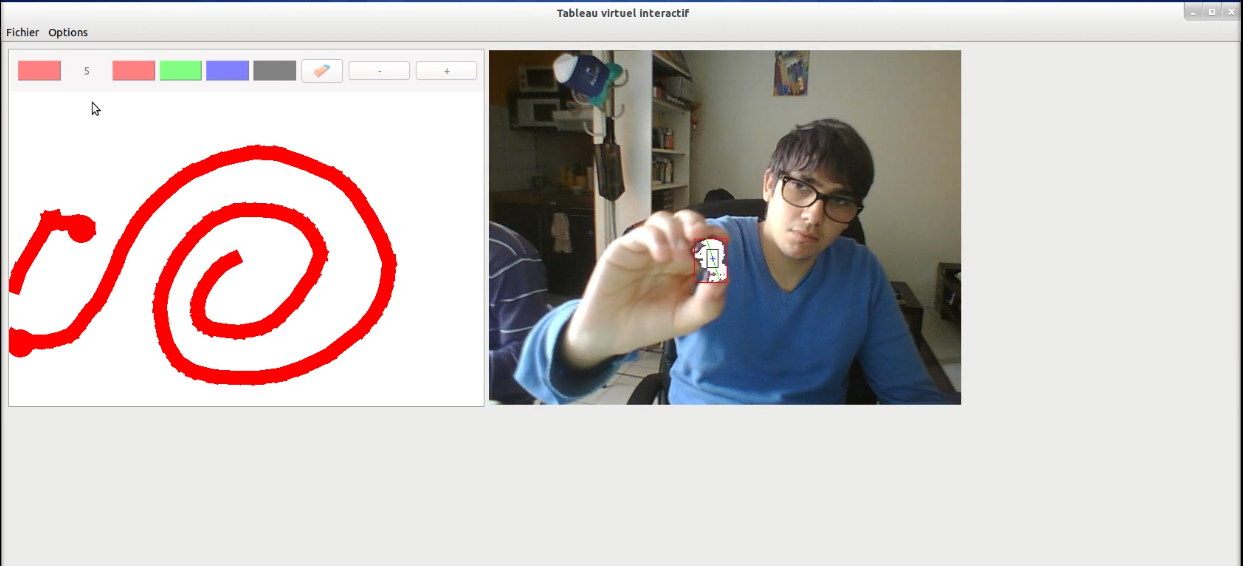
\includegraphics[scale=0.3]{../images/capture-intro.png}\\
			\caption{Aperçu de l'application}
			\label{Aperçu de l'application}
		\end{figure}
	\newpage
		\section{Contexte}
		% TODO
		\paragraph{}
		Ce projet est réalisé dans le cadre des TER (Travaux d'Étude et de Recherche) de 1ère année de Master informatique à L'Université Montpellier 2. \\
		Le TER est un projet qui se déroule sur un semestre, généralement choisi par les étudiants parmi une liste de projets qui leurs sont proposés. \\Ce genre de projet apporte beaucoup aux étudiants. Il leur permet d'une part de travailler une longue période sur un seul et même sujet afin d'obtenir quelque chose de complet, d'abouti. \\D'autre part, le TER (comme son nom l'indique) apporte une bonne expérience dans le domaine de la recherche. En effet, un travail préalable doit être effectué sur l'existant (Est-ce que d'autres projets de ce genre existent? Si oui qu'ont-ils de différent?, etc.), mais également sur la faisabilité (Est-ce possible à faire? Quels algorithmes existent pour répondre à tel ou tel besoin?, etc.).
		\paragraph{}
		La particularité de ce projet réside dans le fait que nous l'avons nous-même proposé à un enseignant-chercheur. Nous avons décidé de proposer ce sujet pour diverses raisons, dont voici les pricipales:
		\begin{itemize}
			\item Tout d'abord, c'est un projet que nous avions en tête depuis plus d'un an, qui a donc eu le temps de murîr et d'être au niveau d'un TER.
			\item Deuxièmement, notre groupe vient de deux formations distinctes : \textbf{AIGLE}, formation orientée génie logiciel ; et \textbf{IMAGINA}, spécialisée dans le jeu vidéo et l'image. Ce projet représentait une manière opportune de lier ces deux spécialités.
			\item Enfin, ce projet était pour nous une bonne occasion de réaliser une application fonctionnelle et distribuable, et par conséquent nous permettre d'explorer une autre facette du développement d'applications : la mise en production.
		\end{itemize}	

	\chapter{Analyse et conception}
		\section{Étude de l'existant et faisabilité}
		\subsubsection{Faisabilité}
		Notre groupe ayant lui-même proposé ce sujet, celui-ci s'accorde parfaitement à nos formations et spécialités. Le choix de ce sujet a donc été réalisé en fonction de nos expériences, savoir-faire et affinités.\\
Ce projet s'inscrivant dans le cadre d'un TER de notre formation, l'étude de la faisabilité n'inclue pas certains critères comme l'étude de marché, le contexte économique ou le besoin réel. 
Nous nous sommes notamment concentrés sur les compétences techniques et de gestion. Pour les parties financement et analyse des coûts, il va sans dire que nous ne disposions d'aucun financement et n'avons donc utilisé que des outils gratuits. \\

		\subsubsection{Existant}
		La vision par ordinateur et particulièrement le suivi d'objets, sont des domaines connus et pour lesquels il existe de nombreux travaux. Nous pouvons nous inspirer de certains de ces travaux afin de proposer des fonctionnalités plus pertinentes, éviter certains écueuils ou plus directement utiliser des outils existants comme la bibliothèque OpenCV.\\
			\begin{itemize}
				\item Exemples dans le jeux vidéo : Kinect, Eye-toy, CamSpace (techniques pour l'IHM, par exemple, mouvements continus ou immobilité sur une zone).
				\item Exemples issus de thèses et de projets de recherche (techniques de programmation).
			\end{itemize}
			\begin{figure}[!h]
				\centering
				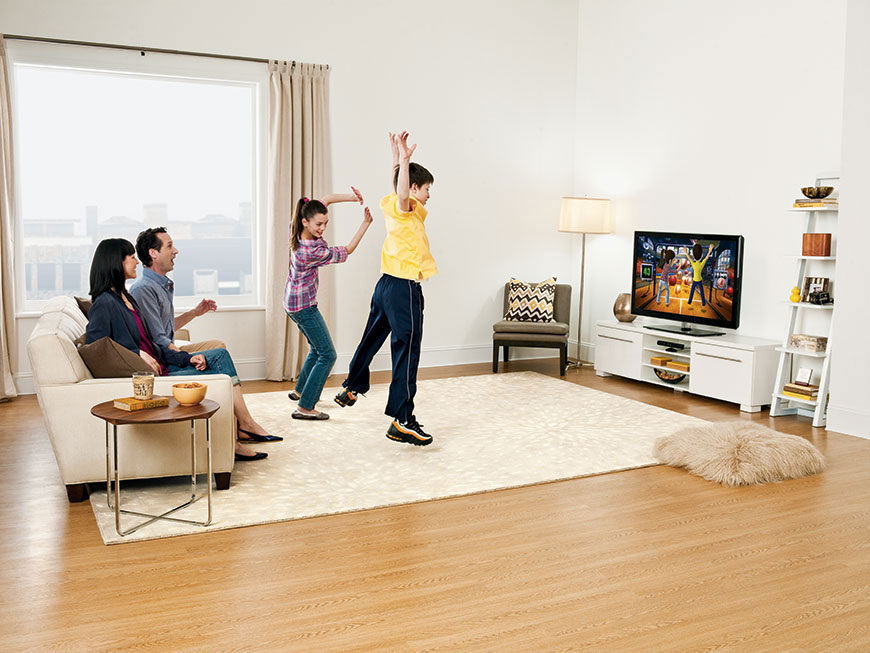
\includegraphics[scale=0.2]{../images/kinect_screen_lg.jpg}\\
				\caption{Exemple du Kinect}
				\label{Exemple du Kinect}
			\end{figure}
		\newpage
		\section{Gestion du projet}
			\subsection{Choix stratégiques}
			\paragraph{}
			Lors de ce projet, nous avons distingué deux parties majeures. La première est une bibliothèque de suivi d'objets. La seconde, une application qui utilise cette bibliothèque pour réaliser un logiciel de dessin interactif. \\
			Ce choix présente plusieurs intérêts :
			\paragraph{}
			Premièrement, ce découpage permet de bien différencier les tâches. Le développement de la bibliothèque requiert des connaissances en \textbf{traitement d'images} pour tracer des couleurs/objets, appliquer des filtres, manipuler les images, etc. Ceci correspond parfaitement à la formation de deux membres du groupe(formation IMAGINA à l'UM2). 
			Le développement de l'application requiert quant à lui des connaissances en \textbf{génie logiciel}, pour l'architecture de l'application, en IHM, pour la réalisation de l'interface (logicielle et gestuelle), ou encore en réseau pour la mise en place de l'architecture client/serveur. 
			Ces différents points correspondent également parfaitement à la formation des deux autres membres du groupe. (Formation AIGLE à l'UM2). Ainsi, les tâches peuvent bien se répartir en fonction des connaissances et spécialités de chacun.
				\paragraph{}
				Deuxièmement, l'intérêt de ce découpage est d'avoir deux projets à la fois complètement indépendants et complémentaires. En effet, la \textbf{bibliothèque} développée offre des fonctionnalités de suivi utilisables par n'importe quelle application.\\
				L'\textbf{application} se charge d'utiliser les fonctionnalités de traitement d'images de la bibliothèque en ajoutant une interface graphique, une couche réseau, une connexion aux webcams ou encore la récupération des images.
				La bibliothèque et l'application sont donc deux projets développés en \textbf{parallèle} et très modulaires. Notre application peut très bien utiliser une autre bibliothèque de traitement d'images, et la bibliothèque peut très bien être utilisée par d'autres applications qui offriraient des fonctionnalités totalement différentes de la nôtre.

			\newpage
			\subsection{Diagramme de Gantt}
			\paragraph{}
			Étant donné que nous avons proposé notre propre sujet, la première étape a été de rédiger un \textbf{cahier des charges} pour définir ce que nous voulions faire et de quelle manière.
			\paragraph{}
			Après ceci, nous avons commencé à effectuer des recherches du côté bibliothèque et application, pour savoir quels outils et techniques utiliser pour arriver à nos objectifs. 
		  Nous avons réservé plusieurs semaines pour effectuer des recherches et perfectionner notre idée du projet. Nous avons donc lu des articles de recherches sur des thématiques proches, effectuer des essais d'outils etc. Cette période d'\textbf{analyse} et de conception sert aussi à penser l'application en imaginant des cas d'utilisations (use cases) et en réalisant le diagramme de classes.

			\paragraph{}
			Par la suite, la majeure partie du temps est réservée au \textbf{développement} en lui même, en prenant en compte la date de présentation du projet pour avoir une réalisation complète. \\  
			Bien entendu ces temps de développement s'accompagnent de réunions avec tout le groupe de projet ainsi que de travail pour lier nos deux sous-parties et les tester ensemble. \\
			Des documents comme le rapport ou la documentation furent produit au fur et à mesure du projet, pour rester en adéquation avec le travail accompli. Voici le rétroplanning qui illustre le déroulement chronologique du projet : \\
				\begin{figure}[!h]
					\centering
					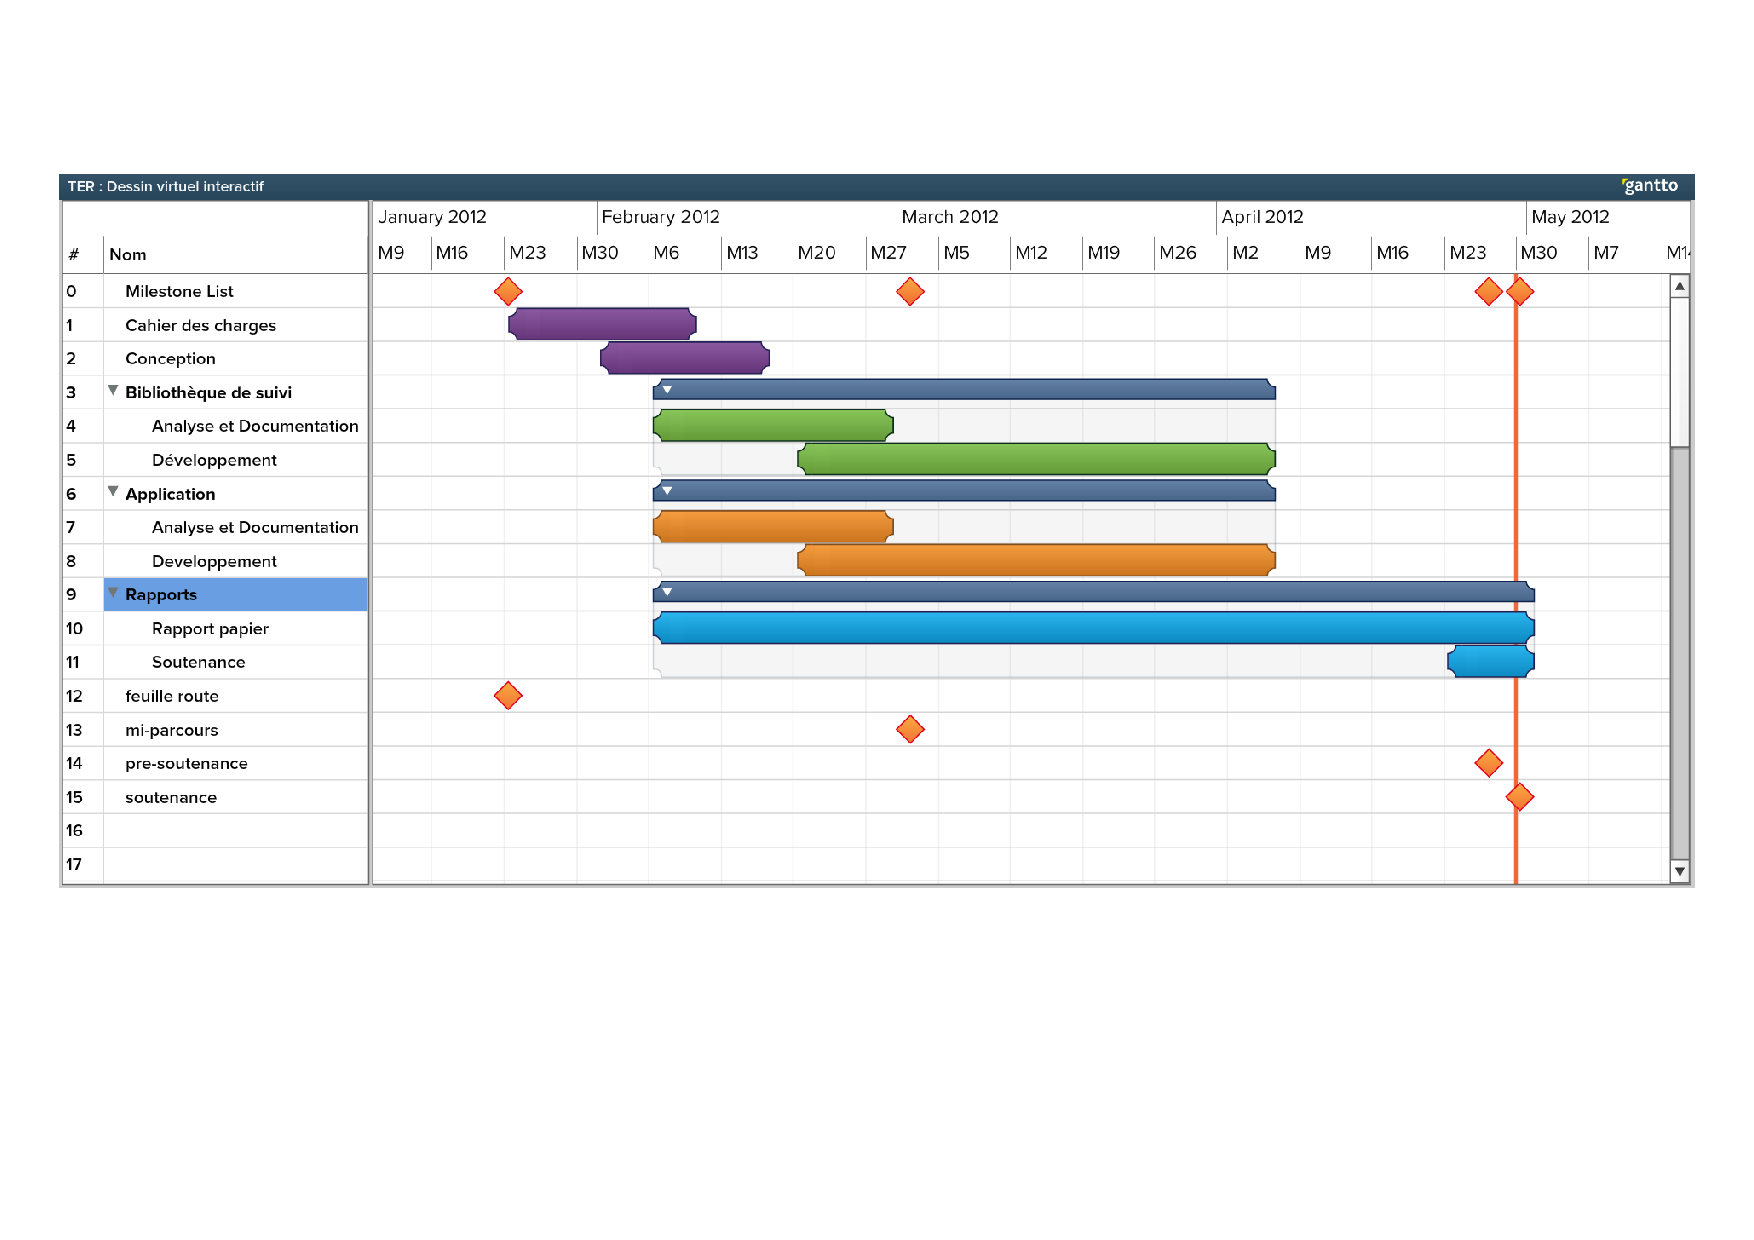
\includegraphics[scale=0.6]{../images/retro-planning.pdf}\\
					\caption{Rétroplanning}
					\label{Rétroplanning}
				\end{figure}
		\newpage
		\section{Outils utilisés}
		Durant la période de recherche et au cours du projet nous avons utilisé différent outils pour nous aider dans la réalisation. Nous les présentons dans cette section. 
			\subsubsection{Outils collaboratifs}
			\paragraph{}
			
\includegraphics[scale=1]{../logos/subversion-logo.png} 
			Subversion : Un gestionnaire de versions qui nous permettant de synchroniser notre travail, de partager le code source et de s'échanger quelques documents complexes (ce rapport par exemple).
			\paragraph{}
			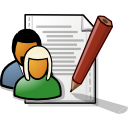
\includegraphics[scale=0.25]{../logos/Gobby-logo.png} 
			Gobby :
			Logiciel libre pour l'édition collaborative, qui permet de développer à distance sur le même document simultanément. \\

			\paragraph{} Bien sûr ces outils ne sont pas suffisants, nous avons donc fait des réunions régulières pour organiser le travail et décider des orientations du projet. Par ailleurs, nous avons beaucoup échangé pour que tout le monde soit toujours au courant des différentes informations importantes.
			
			\subsubsection{Outils techniques}
			\paragraph{} Nous avons utilisé le système d'exploitation LINUX tout au long du projet, pour des raisons idéologiques d'une part et d'autre part pour les nombreux outils de développements qu'il offre. Le projet étant réalisé avec des librairies existantes sous plusieurs autres systèmes, en théorie la portabilité de l'application n'est pas bornée à LINUX.
			
			\paragraph{} Par ailleurs, nous avons utilisés divers logiciels tels que Dia et Umbrello pour faire respectivement les diagrammes de séquences, et les diagrammes de classes et les cas d'utilisations. \\
			Nous avons aussi utilisé qmake pour générer les makefile et le compilateur g++ pour tout le projet, nous n'avons pas utilisé d'IDE mais parfois valgrind ou gdb pour déboguer. \\
			Quelques schémas ont été réalisés avec LibreOffice et Gimp. \\
			\subsubsection{Langages :}
			\paragraph{} Langage C pour la bibliothèque : ce langage est bien adapté à la réalisation d'une bibliothèque car il permet l'écriture de fonctions. Par ailleurs c'est un langage bien adapté au domaine du traitement de l'image car il est de bas niveau, et très rapide. De plus, nous avons utilisé des bibliothèques (OpenCV par exemple) qui ont été écrites initialement en C.
			\paragraph{} Langage C++ pour l'application : c'est un langage objet ce qui nous aidait pour la conception. Il est également très rapide et c'est un langage avec lequel nous sommes à l'aise et avons de l'expérience, ce qui nous évitait de devoir apprendre un nouveau langange, et par là de perdre un temps précieux.\\
			
			\subsubsection{Bibliothèques :}
			
\includegraphics[scale=0.15]{../logos/qt_logo.png}
			Qt : bibliothèque d'IHM (et bien plus) en C++, nous aide pour faire les interfaces graphiques, pour la partie réseau également où elle offre des abstractions agréables. \\
			\paragraph{}
			
\includegraphics[scale=1]{../logos/OpenCV_Logo.png}
			: bibliothèque de traitement de l'image, nous aide à exploiter la webcam et pour le traitement de l'image avec plusieurs fonctionnalités. \\
		
		\newpage
		\section{Analyse}
			\subsection{Cas d'utilisations}
				\begin{figure}[!h]
						\centering
						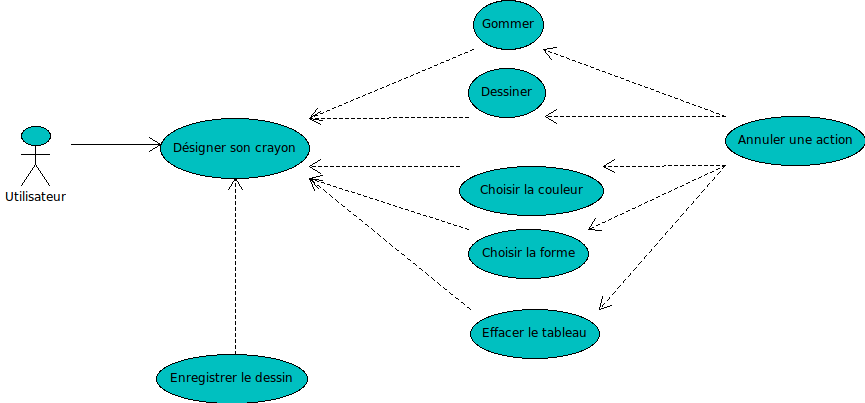
\includegraphics[scale=0.6]{../images/Dessin.png}\\
						\caption{Cas d'utilisation dessin}
						\label{Cas d'utilisation}
				\end{figure}
				
				Ce cas d'utilisations présente rapidement les différentes fonctionnalités que nous voulions implémenter.
				\begin{itemize}
				\item Dessiner sur le tableau
				\item Gommer
				\item Choisir la couleur du pinceau
				\item Choisir l'épaisseur du pinceau
				\item Effacer complètement le tableau
				\item Enregistrer le dessin
				\end{itemize}
				\ \\
				Nous avions également envisagé de développer un outil permettant de revenir en arrière, nous ne l'avons pas fait dans la version finale. \\
			\newpage
			\subsection{Diagrammes de séquences}
			Les diagrammes qui suivent expliquent le fonctionnement de l'application pour l'utilisation en local et l'utilisation en réseau.
			\subsubsection{Fonctionnement en local}
				\begin{figure}[!h]
						\centering
						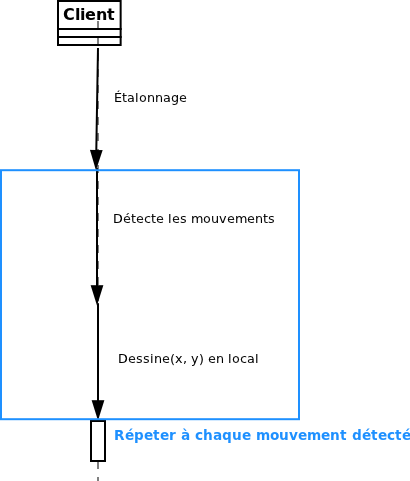
\includegraphics[scale=0.6]{../images/sequence_local.png}\\
						\caption{Diagramme de séquence local}
						\label{Diagramme de séquence local}
				\end{figure}
				\paragraph{}
				On peut voir sur ce diagramme que le fonctionnement en local est assez basique. Dans un premier temps, l'utilisateur \textbf{étalonne} l'objet avec lequel il veut dessiner. Ensuite, lorsque l'utilisateur déplace l'objet en question, l'application \textbf{détecte} ce déplacement, et \textbf{dessine} à la nouvelle position de l'objet. Ce schéma de détection-dessin est répété jusqu'à fermeture de l'application. \\
				Ainsi, l'utilisateur verra se dessiner chacun des mouvements qu'il effectue avec son objet.

				\newpage
				\subsubsection{Fonctionnement en réseau}
				En réseau, l'utilisation suit le même schéma, mais un autre acteur entre en jeu, le \textbf{serveur}.
				\begin{figure}[!h]
						\centering
						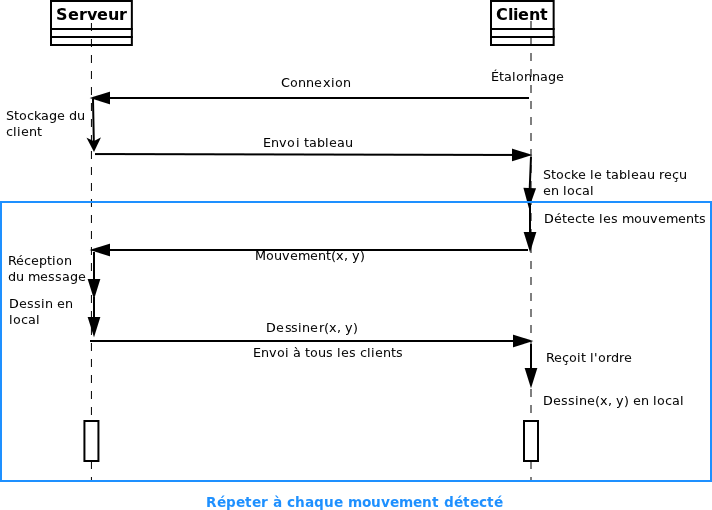
\includegraphics[scale=0.62]{../images/sequence_reseau.png}\\
						\caption{Diagramme de séquence réseau}
						\label{Diagramme de séquence réseau}
				\end{figure}
				\paragraph{}
				Comme pour une utilisation locale, l'utilisateur commence par \textbf{étalonner} l'objet à suivre. Puis, la connexion s'effectue auprès du serveur, qui va renvoyer le dessin courant au nouveau client. Une fois en possession du dessin, le client le stocke et peut rentrer dans la boucle de détection-dessin.
				\paragraph{}
				Comme en local, l'application va \textbf{détecter} le mouvement de l'objet suivi. La nouvelle position est envoyée au serveur qui va dessiner sur son propre tableau, puis renvoyer à tous les clients l'ordre de \textbf{dessiner} à cette même position. Chaque client verra donc ce que les autres clients dessinent. \\
				Ainsi, l'utilisateur verra se dessiner chacun des mouvements qu'il effectue avec son objet, mais également ceux de tous les autres clients.
				\paragraph{}
				On peut donc voir que pour l'utilisateur, le fonctionnement est identique qu'il dessine seul ou avec d'autres personnes :
				\begin{itemize}
					\item Il étalonne l'objet
					\item Il déplace l'objet
					\item l'objet dessine sur le tableau
				\end{itemize}
				Cependant, dans la pratique, le fonctionnement n'est pas le même. En réseau, chaque mouvement passe par le serveur qui se charge de faire le lien avec tous les clients de l'application.

			\newpage
			\subsection{Diagrammes de classes}
				La bibliothèque fonctionne grâce à la manipulation d'un curseur qui correspond en fait au curseur, ou objet, physique manipulé par l'utilisateur.
				Le curseur est représenté en mémoire sous la forme d'une strucure de données \textbf{\textit{Cursor}}. On utilise donc des informations telles que la taille de ce curseur, sa position ou encore sa couleur.\\
				Cette structure de données est engendrée par la fonction \textit{\textbf{calibration}} de la bibliothèque. Elle est ensuite utilisée par la fonction \textit{\textbf{track}}, qui permet la mise à jour des informations relatives au curseur par rapport à une image. \textit{Cursor} sert aussi à intéragir avec les suivis, elle permet donc de régler certain attributs comme des seuils de tolérance par exemple. \\
				\begin{figure}[!h]
						\centering
						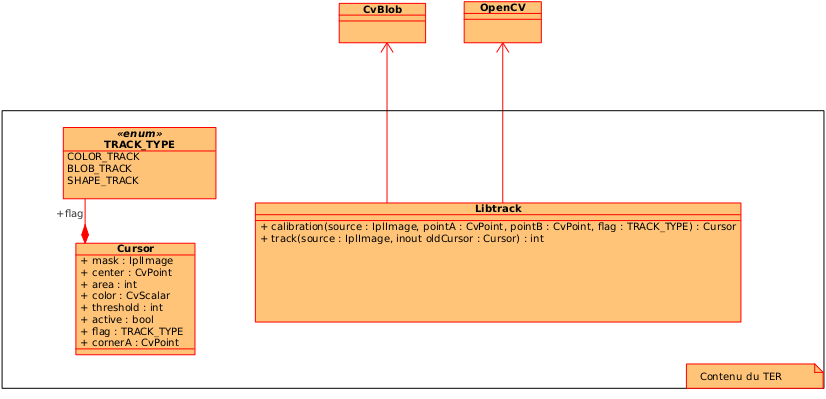
\includegraphics[scale=0.8]{../images/libtrack-uml.png}\\
						\caption{Architecture de la bibliothèque}
						\label{Architecture de la bibliothèque}
				\end{figure}
				

				La bibliothèque dépend de deux bibliothèques externes:
				\begin{itemize}
					\item OpenCV, spécialisée dans le traitement des images
					\item CvBlob, bibliothèque issue d'OpenCV utlisée pour la recherche d'objet dans des images binaires
				\end{itemize}

				\newpage			
				Le diagramme qui suit vous présente l'architecture de notre application. \\
Avant de commencer l'application, nous avons décidé de passer un long moment sur la réflexion pour avoir une architecture solide et modulable.\\Nous avons dans un premier temps identifié les différents modules dont serait composée notre application et quels étaient précisément le ou les rôles de chacun. \\Ensuite, nous avons réfléchi à quel était le meilleur moyen pour que ces différents modules puissent communiquer en évitant toute redondance ou communication superflue. \\Une fois cette réflexion faite, nous avons dessiné le diagramme suivant : \\
				\begin{figure}[!h]
						\centering
						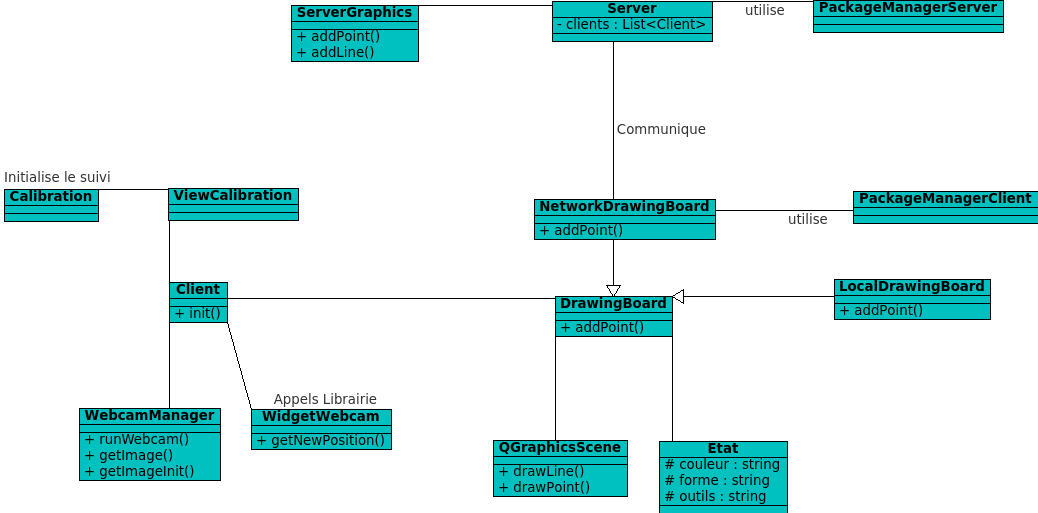
\includegraphics[scale=0.6]{../uml/classes.png}\\
						\caption{Pseudo-Diagramme de classe de l'application}
						\label{Pseudo-Diagramme de classe de l'application}
				\end{figure}
				
				On peut identifier quatre modules principaux : \\
				\begin{itemize}
					\item \textbf{Le module d'étalonnage} (Calibration et ViewCalibration). Ce module sert à tout ce qui touche à l'étalonnage de l'objet. Une fois qu'il est effectué, le module va appeler le module \textit{client} pour lui signaler que l'étalonnage est fait, et lui envoyer les informations qui correspondent (objet à suivre, type de suivi, dessin en local ou réseau, etc.)
					\item \textbf{Le module client} (Client). Ce module qui est le coeur de l'application possède deux rôles principaux. Il va dans un premier temps construire toute l'interface graphique (tout ce qui est visuel) qui sera présentée à l'utilisateur. C'est aussi lui qui va assurer la communication entre tous les autres modules locaux dont il est le seul intermédiaire.
					\item \textbf{Le module de dessin} (DrawingBoard, LocalDrawingBoard et NetworkDrawingBoard). Ce module a également deux rôles. Il va s'occuper de toute la partie dessin (stocke la couleur et taille du pinceau, dessine les points, lignes, etc.). Aussi, pour une utilisation en réseau, c'est lui qui va se charger de communiquer avec l'application serveur.
					\item \textbf{Le module serveur} (Server, ServerGraphics). C'est ce module qui met en relation les différents client et qui synchronise le dessin. Il reçoit les ordres de dessin, les stocke et les renvoie à tous les autres clients.
				\end{itemize}
				\ \\
				La classe \textbf{WebcamManager} est la seule classe qui va communiquer avec le \textbf{matériel} (ici les webcams). Lorsque l'on veut une nouvelle image de la webcam, le module client va demander à WebcamManager la nouvelle image et l'envoyer au module qui en a besoin. \\
				La classe \textbf{WidgetWebcam} est la seule classe qui va communiquer avec la \textbf{bibliothèque de suivi}. \\
				Les classes QGraphicsScene et Etat représentent respectivement le dessin et l'état actuel du pinceau. \\
				Les classes PackageManager* servent à assembler et désassembler les paquets qui transitent sur le réseau.
				\newpage
				\paragraph{Scénario :} \ \\
				Afin d'illustrer la modularité de notre application, on pourrait imaginer le scénario suivant :
				\begin{itemize}
					\item L'étalonnage s'effectue. Une fois terminé, le module d'étalonnage va prévenir le client et lui donner les informations.
					\item Chaque X millisecondes, le client va interroger WebcamManager pour obtenir une nouvelle image.
					\item Le client va envoyer cette image à WidgetWebcam pour obtenir la nouvelle position. (Grâce à la bibliothèque de suivi)
					\item Le client va maintenant envoyer cette position à DrawingBoard qui va dessiner le nouveau point en fonction de la couleur la taille, etc.
				\end{itemize}
				On voit ici que chaque module rempli bien son rôle et assure le bon fonctionnement général de l'application.
				
				$$$$ \\
				Une fois cette phase de réflexion terminée, toute l'architecture de la bibliothèque et de l'application était pensée et écrite. \\
				Nous pouvions alors débuter la phase de réalisation, programmer et imbriquer les différents modules et  nous attaquer aux problèmes plus techniques.

				
	
	\chapter{Réalisation}
		\section{Bibliothèque de suivi}
			Cette partie du développement a pour objectif de fournir un ensemble de fonctionnalités permettant la \textbf{reconnaissance} et le suivi d'un objet, que nous appellerons \textbf{Curseur}, à partir d'images. \\
			L'objectif est de développer notre propre \textbf{bibliothèque} pour d'une part avoir un outil remplissant précisément nos objectifs et d'autre part de faire un travail de recherche et développement dans le domaine du traitement de l'image (en particulier le suivi d'objets). \\
			Un certain nombre de bibliothèques existantes proposent des outils de reconnaissance de formes, de suivis de modèle ou d'évaluation de composantes connexes. Le travail consiste donc à tirer partie de ces bibliothèques en les associant de manière à proposer des méthodes efficaces et simples à utiliser. Cela implique une bonne connaissance des outils existants, de leur compréhension et de leur utilisation conjointe dans le but de concevoir notre propre bibliothèque.
			\newpage
				\subsection{Aspect général}
				La structure générale de la bibliothèque est relativement \textbf{simple} à appréhender, ce qui permet une utilisation aisée sans connaissances particulières en traitement d'images. Comme expliqué dans la partie d'analyse, le fonctionnement de la bibliothèque de suivi repose sur l'utilisation d'une structure de données \textbf{\textit{Cursor}} créée et manipulée respectivement par les deux fonctions \textcolor{blue}{d'étalonnage} et \textcolor{orange}{de suivi}.
				\paragraph{} Notre biliothèque dispose de diverses méthodes de suivi pour \textbf{enrichir} l'offre disponible pour l'utilisateur. C'était évidemment aussi pour nous le moyen d'\textbf{étudier} différentes méthodes et de pouvoir les \textbf{comparer}. Il faut cependant ici faire la distinction entre le point de vue de l'utilisateur et celui du développeur. En effet, si certaines méthodes peuvent apparaitre différentes par leur utilisation ou l'expérience qu'elles procurent, elles peuvent être très proches techniquement.
				\paragraph{}Ainsi, notre bibliothèque propose actuellement trois types de suivi différents : par couleur simple, par composantes connexes ou par modèle. Mais d'un point de vue technique et réalisation, nous pouvons regrouper les deux premières car s'appuyant toutes deux sur une recherche par couleur, comme nous le verrons en abordant leur fonctionnement.\\
				\begin{itemize}
\item {\textcolor{marron}{par modèle} : } Ici, c'est la forme de l'objet qui est utilisée. On recherche une correspondance forte entre un pattern de l'objet recherchéet une éventuelle zone solution dans l'image. \\
\item {\textcolor{vert}{par couleur} : } On s'intéresse ici aux valeurs des couleurs (des pixels) de l'objet plutôt qu'à leur disposition spatiale. Des méthodes d'échantillonage et de seuillage permettent de proposer un résultat plus fin et plus souple qu'une moyenne de couleur seule. Cette dernière ne peut en effet supporter des variations de teinte fortes au sein de l'objet.
				\end{itemize}
							
				\begin{tabbing}
				\=L'affinage de la \=recherche et le choix par l'utilisateur du type de suivi à réaliser passe par la manipulation d'une énumération,\\ \>proposée par la bibliothèque. Aujourd'hui composée de 3 éléments correspondant chacun à un type de suivi particulier, cette\\ \>énumération est amenée à s'agrandir avec l'ajout de nouvelles méthodes. \\
				\>\>\begin{itshape}enum TYPE\_TRACK \{TRACK\_COLOR, TRACK\_SHAPE, TRACK\_BLOB\};\end{itshape}
				\end{tabbing}
				\quad 
				\quad Il convient aussi de noter que l'utilisation de la biliothèque de suivi implique de fournir une image sous le format IplImage d'OpenCV, que nous avons utilisé.
				\newpage
				\subsubsection{\textcolor{blue}{A) Étalonnage}} \paragraph{}
				Afin d'effectuer le suivi d'un objet (au sens large du terme) grâce à notre bibliothèque, il convient en premier lieu de faire appel à la fonction \textit{calibration}. Réalisant l'étalonnage, elle permet de créer et d'initialiser la struture de suivi, appelée \textbf{\textit{Cursor}}, contenant l'intégralité des informations qui vont permettre d'identifier l'objet et de réaliser sa localisation dans les images futures. C'est lors de cette étape que l'utilisateur doit préciser le type de suivi soubaité, par l'intermédiaire d'un simple paramètre.
					\paragraph{Utilisation}
					\begin{tabbing}
					\quad Du point de \=vue de l'utilisateur, une seule fonction permet de gérer la totalité de l'étalonnage, ce qui permet de simplifier\\ l'utilisation de notre bibliothèque : \\
					\>\begin{itshape}Cursor * calibration(IplImage * source, CvPoint A, CvPoint B, TYPE\_TRACK flag);\end{itshape}
					\end {tabbing}
					\quad Cette fonction, créant et initialisant la structure de suivi, n'est en réalité qu'une \textbf{enveloppe} faisant appel à une fonction différente selon le \textit{flag} envoyé. Ces différences permettent de préparer la structure aux spécificités des fonctions de track et d'optimiser le suivi. Il suffit donc de lui passer l'image où se trouve l'objet, deux points pour définir ses contours et enfin un \textit{flag} déterminant la méthode à employer, à choisir parmi les objets de l'énumération.
					\paragraph{Fonctionnement} \paragraph{}
					Pour réaliser l'étalonnage, on commence par créer et initialiser la structure de suivi Cursor en utilisant les informations recueillies lors de l'appel de la fonction. C'est donc lors de cette étape que l'on fixe le type de suivi souhaité et que l'on détermine le masque correspondant à l'objet, son aire, son centre ou encore son seuil.\\
					On fait alors appel, en fonction du type de track, aux différentes sous-fonctions d'étalonnage. Celles-ci, plus complexes, utilisent des notions de traitement d'image que nous détaillerons dans la partie technique.\\
					\begin{itemize}
						\item{\textcolor{vert}{Couleur}}\\
						Pour ces deux méthodes, on commence par transformer l'image source BGR (Blue Green Red) en HSV (Hue Saturation Value) afin de mieux traiter les problèmes d'éclairage et de saturation des couleurs. On fait ensuite appel une fonction \textit{mainColor} afin de déterminer la couleur principale de l'objet à suivre. A noter qu'il serait ici possible d'utiliser une autre méthode pour déterminer la couleur à suivre, comme la couleur du pixel central de l'objet, ou la moyenne de couleur avec \textit{colorAverage} par exemple.
						\\\item{\textcolor{marron}{Modèle}}\\
						On crée un masque contenant la sous-image que forme l'objet à suivre parmi le reste de l'image source. Celui-ci servira ensuite de template que l'on cherchera à retrouver dans les nouvelles images entrantes lors du suivi.
					\end{itemize}
					\newpage
				\subsubsection{\textcolor{orange}{B) Suivi d'un objet}} \paragraph{}
				Une fois ces informations enregistrées, il est alors possible de réaliser le suivi de notre objet au travers de nouvelles images. On fait ainsi appel autant de fois que nécessaire à la fonction \textit{track} de suivi, afin mettre à jour la structure de données avec les modifications inhérantes au changement d'image, comme la nouvelle localisation de l'objet par exemple.
						\paragraph{Utilisation}
						\begin{tabbing}\quad De la même ma\=nière, cette fonction unique permet de simplifier l'utilisation de la bibliothèque : \\
						\> \begin{itshape}int track(IplImage * source, Cursor * oldCursor)\end{itshape}
						\end{tabbing}
						\quad En effet, la fonction se charge de faire appel aux différentes méthodes nécessaires à la réalisation du suivi désiré de l'objet. Il suffit de lui fournir la structure de données contenant toutes les informations importantes, et le nouveau contexte avec une image. On peut noter que la fonction renvoie un entier permettant de s'assurer de son bon fonctionnement.
						\paragraph{Fonctionnement}\paragraph{}
						Comme expliqué précédemment, il faut en fait différencier deux types de suivi : le suivi par couleur et celui par modèle. Ceci est bien sur invisible pour l'utilisateur qui voit lui bien trois types disctincts : par barycentre simple, par composantes connexes et par modèle.\\
						\begin{itemize}
							\item{\textcolor{vert}{Couleur}}\\
							La première étape consiste à \textbf{binariser} l'image source en utilisant la valeur de seuillage portée par le Cursor, grâce à la méthode \textit{binarisation}. De cette manière, on obtient une image binaire où les points blanc correspondent aux pixels dont la couleur est proche de celle recherchée, et les noirs aux zones non pertinentes. Ensuite, l'idée est de calculer le \textbf{barycentre} des zones ainsi selectionnées comme pertinentes. C'est sur ce point que diffère les deux méthodes par couleur. La première calcule le barycentre sur la totalité de ces pixels blanc grâce à la méthode \textit{setNewCentroid}. La seconde va d'abord déterminer l'ensemble des composantes connexes de ces pixels puis effectuer le calcul du barycentre de la zone la plus importante, à priori la plus pertinente donc. Elle utilise pour cela la méthode \textit{blobFounding}.
Pour rappel, une forme est connexe si elle est faite d'un seul morceau, une composante connexe étant donc un tel objet perçu sur l'image binaire.\\
							\item{\textcolor{marron}{Modèle}}\\
							L'idée est de rechercher une \textbf{correspondance} forte entre le pattern de l'objet recherché et l'image source. Pour cela, on pose des calques de l'objet modèle à intervalle régulier sur l'image entrante, et on compare le taux de ressemblance afin d'évaluer la correspondance. C'est donc à l'endroit où ce taux sera le plus important que l'on pourra localiser notre objet. Il faut cependant penser à obtenir une valeur minimale pour ne pas réaliser de fausse détection. Tout cela est réalisé grâce à la fonction \textit{shapeTrack}.
						\end{itemize}
						\newpage
				\subsection{Fonctionnement technique}
					Voici le détail de fonctionnement de quelques fonctions clés de la bibliothèque, on peut ici distinguer deux types de fonctions : les fonctions d'\textcolor{blue}{étalonnage} et celles de \textcolor{orange}{suivi}.
					\subsubsection{\textcolor{blue}{Fonctions d'étalonnage}}
						Pour l'utilisation des suivis par couleur, nous avons besoin d'avoir la couleur de l'objet à suivre. Dans cette optique nous avons utilisé trois manières de l'extraire.
						\paragraph{centricPixel} \paragraph{}
						Cette méthode est la première que nous avons utilisée, elle prend simplement la couleur du pixel au \textbf{centre} de l'objet suivi. Cette méthode fonctionne assez bien avec les objets ayant de grandes aires colorées avec peu de changement de saturation, ce qui n'est pas suffisant dans le cadre de notre projet.
						\paragraph{colorAverage} \paragraph{}
						\textit{colorAverage} est plus élaborée que la méthode précedente. En effet, elle calcule la couleur \textbf{moyenne} dans une boîte englobante autour de l'objet, ce qui permet donc d'obtenir une couleur plus représentatrice de l'objet. Celle-ci fonctionne alors sur les objets unicolores et est moins sensible au changement de valeur des couleurs de l'image. Par contre, cette fonction ne fonctionne absolument pas avec les objets multicolores, la moyenne de couleur n'ayant pas de sens sur ceux-ci.
						\paragraph{mainColor} \paragraph{}
						\textit{mainColor} est donc la dernière fonction d'extration de couleur que nous avons dévéloppée. Celle-ci fonctionne sur les objets multicolores (ayant tout de même de grandes aires unicolores) et est aussi peu sensible au changement de valeurs.\\
						Elle se déroule en deux étapes : la recherche de la couleur dominante, puis la moyenne des couleurs proches de celle-ci. \\Tout d'abord, on construit l'\textbf{histogramme} des couleurs dans la sous-image, par tranche de 10 degrés, puis on récupère la tranche la plus représentée.\\
Ensuite, on parcourt une nouvelle fois la sous-image en faisant la \textbf{moyenne} des H, S et V des pixels appartant à la tranche de couleur prédominante.

						
						\paragraph{Binarisation} \paragraph{}
							Une fois cette couleur, que nous appellerons couleur étalon, extraite, nous pouvons l'utiliser pour créer l'\textbf{image binaire} nécessaire au suivi par couleur. Cette image est une image en noir et blanc, où le blanc représente les points retenus par les fonctions précédentes. Ces zones blanches nous permettrons ensuite de calculer la position de notre objet, par l'utilisation de méthodes interprétant ce type d'images.\\
							Le principe de cette fonction est donc assez simple. On construit d'abord une nouvelle image de la même taille que l'image source. Puis, pour chaque pixel, si sa couleur originale est assez proche de la couleur étalon, on le passe à blanc, sinon en noir. La notion de "assez proche de la couleur" est parametrée par une variable de tolérance, \textit{threshold}, pouvant être réglée par le biais de la structure \textbf{\textit{Cursor}}.\\
							Enfin, avant de retourner cette nouvelle image binaire, on lui applique une série de \textbf{fermetures}. Le principe de la fermeture est d'appliquer une \textbf{\textcolor{vert}{érosion}} puis une \textbf{\textcolor{red}{dilatation}} des formes blanches obtenues. L'intérêt de cette action est d'éliminer les éventuels pixels blanc solitaires sur l'image, de manière à diminuer au maximum les parasites sur l'image qui viendraient fausser les opérations à venir.
					\newpage
					\subsubsection{\textcolor{orange}{Fonctions de suivi}}
						\paragraph{setNewCoord} \paragraph{}
						Le fonctionnement de cette méthode plutôt simple, on parcourt l'\textbf{image binaire} issue de la binarisation en faisant la somme des positions en X et en Y des pixels blanc. Par division de ces sommes par le nombre de pixels présents sur l'image, on obtient le barycentre du blanc sur celle-ci. La précision de cette position est variable en fonction de la qualité de l'image binaire : un grand nombre de parasites (ou artefacts) faussera la précision de cette méthode.\\
						D'autre part, en comparant le nombre de pixels blanc présents sur l'image avec celui de l'étalonnage, on peut en déduire si l'objet a été approché ou éloigné. En fonction de cela, on peut affecter l'état du curseur, actif ou non. C'est une manière de proposer une détection d'action intuitive.
						\paragraph{blobFounding} \paragraph{}
						Le fonctionnement de cette fonction est assez similaire à celui de \textbf{setNewCoord} mais permet une détection beaucoup plus précise. On part ici aussi de l'image binaire engendrée par \textbf{Binarisation}, mais au lieu de calculer le barycentre de l'image, on va d'abord effectuer une  \textbf{recherche de composantes connexes} sur l'image. Une telle forme sur l'image binaire aura l'allure d'une tâche blanche, le but étant d'\textbf{isoler} chacune de ces "tâches" de manière à pouvoir déterminer laquelle représente notre objet. Ensuite, on calcule le barycentre de cet objet et on obtient alors la nouvelle position de notre curseur. D'autre part, on compare l'aire de l'objet avec son aire au "repos" (son aire à l'étalonnage). Si celle-ci est suffisamment augmentée, on en déduit que l'objet a été approché, et par la que curseur est à l'\textbf{état actif}\\
						L'avantage de cette fonction par rapport à la précédente est qu'elle permet d'\textbf{éliminer} les parasites n'ayant pas été effacés par la fermeture effectuée sur l'image binaire.
						\paragraph{shapeTrack} \paragraph{}
						Cette dernière méthode utilise la comparaison de modèle. Le principe est assez simple, on dispose d'une image, ou \textbf{scène}, et d'une deuxième image, le \textbf{modèle}. A partir de ceci, la fonction va essayer de placer le modèle partout sur la scène. On récupère en sortie une image en niveau de gris, la \textbf{matrice probabiliste}.\\Les dimensions de cette image résultat sont directement liées à celles de l'image initiale (W*H) et de l'image modèle (w*h) telles que dim(resultat) =  (W-w+1)* (H-h+1). Cela est bien sur du au fait qu'on ne puisse pas "poser" le masque modèle pour comparaison sur une zone de l'image initiale où il ne pourrait rentrer entièrement.\\ Sur cette image, chaque pixel ou case, possède une valeur entre 0 et 255. Plus un pixel est proche de 255, ou blanc, plus cela veut dire que les chances que le modèle se trouve à cet endroit de la scène est grand. Une deuxième fonction permet alors, après une remise à l'echelle, d'extraire de cette matrice la position la plus probable du modèle.
\newpage
						
		\section{Application}
	\paragraph{Application :\\}
L'application doit exploiter le plus efficacement possible la bibliothèque de reconnaissance. Nous voulons donc mettre en place un étalonnage de l'objet à suivre le plus précisément possible. Le projet doit ensuite être exploitable et utile, nous devons donc mettre en place un certain nombre d'outils tels que la possibilité de gommer, changer de forme, de couleur etc. 
Un module réseau est aussi prévu pour une utilisation concurrente et synchronisée. Et bien sûr la fonctionnalité clé de l'application est le tableau virtuel, qui devra donc être exploitable et le dessin devra être fidèle aux mouvements reconnus.

		\subsection{Interface graphique}
			Nous avons fait le choix de découper notre interface graphique en deux parties. La première permet à l'utilisateur d'effectuer certaines actions à la souris, la seconde lui permet d'effectuer des actions de manière gestuelle. \\
			Nous avons également choisi de créer une interface très intuitive, l'utilisateur ouvre l'application et sait tout de suite comment interagir avec le programme, et quelles sont les fonctionnalités qui lui sont proposées. \\
			Dans un premier temps, l'utilisateur est guidé par une interface de type précédent-suivant qui permet de bien l'assister pour configurer l'objet que le programme va suivre. Ensuite, l'utilisateur voit s'afficher l'application.
			\subsubsection{Classique}
				L'interface que nous apellons "classique" désigne le genre d'interface que l'on retrouve dans toute sorte d'application bureautique. Avant de la développer, nous avons fait un schéma simple représentant une telle interface adaptée à notre programme : \\
			\begin{figure}[!h]
						\centering
						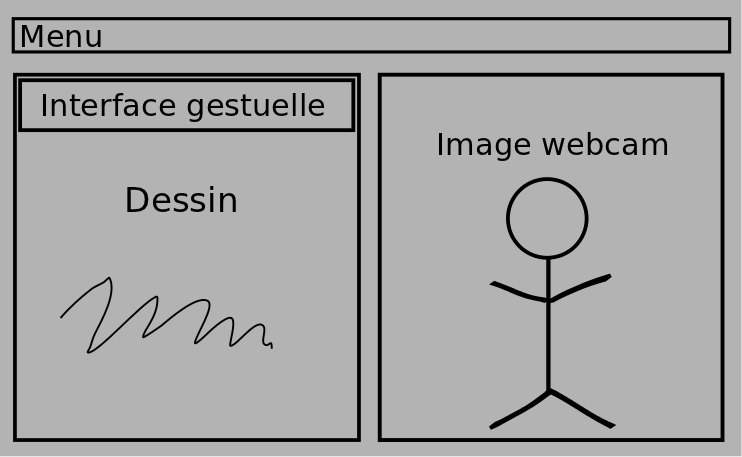
\includegraphics[scale=0.4]{../images/interface.png}\\
						\caption{Interface de dessin}
						\label{Interface de dessin}
			\end{figure}
			
			On peut voir sur la partie haute un menu tel qu'on en trouve dans tout type d'applications bureautiques. Ce menu est divisé en deux catégories au nommage conventionnel (Fichier, Option). \\
			Dans ce menu, les actions sont également familières pour l'utilisateur : Enregistrer, Quiter. \\
			Toujours dans cet esprit d'intuitivité, nous avons assigné des raccourcis usuels à chacune de ces actions (Ctrl+S pour la sauvegarde, Ctrl+Q pour quitter, etc.)
			
			\subsubsection{Gestuelle}
				L'utilisateur qui est en train de dessiner n'a pas forcément envie de reprendre la souris pour pouvoir changer la couleur ou la taille de son pinceau. Nous avons donc imaginé une interface, toujours naturelle, qui permettrait à l'utilisateur de pouvoir agir sur son dessin directement par ses gestes. \\
				Ainsi, l'utilisateur n'aurait qu'à reculer la main pour passer en mode "passif" et positionner l'objet sur les boutons de l'interface pour interagir avec l'application. \\
				Le fait de ne pas proposer toutes les fonctionnalités depuis cette interface est un choix voulu. En effet, on imagine qu'il serait dommage que d'un seul geste rapide, l'utilisateur efface malencontreusement l'intégralité de son dessin. 
		\subsection{Fonctionnalités}
			\subsubsection{Actions}
				Pour augmenter l'utilisabilité du logiciel, nous avons décidé de développer différentes actions permettant à l'utilisateur de directement interagir avec son application. \\
				\begin{itemize}
					\item \textbf{Clic :} Dès le début du projet, nous avons fait le choix de proposer le clic à l'utilisateur. L'idée est ici de mettre à disposition deux modes à l'utilisateur. Le \textbf{mode dessin}, activé quand l'utilisateur approche l'objet de la camera, fera que chaque mouvement d'objet dessinera à l'écran. Le \textbf{mode main levée}, activé quand l'utilisateur éloigne l'objet de l'écran, fera que les mouvements ne dessinent plus sur le tableau. Cependant, l'utilisateur verra, grâce à un curseur, la position de son objet sur le tableau. Grâce à ces deux modes, l'utilisateur pourra dessiner sur le tableau, puis arêter quand il le souhaite ce dessin pour aller sélectionner un bouton sur l'interface gestuelle.
					\item \textbf{Sauvegarde : } Le but principal était de permettre de dessiner sur un tableau. Il nous fallait ensuite rendre ce dessin exploitable. Nous avons donc décidé de developper une action qui permettrait à l'utilisateur de sauvegarder l'état du tableau sous forme d'image pour ensuite l'exploiter à l'aide d'un autre logiciel, ou autre.
					\item \textbf{Plein écran : } Afin que l'utilisateur puisse plus facilement dessiner, nous avons également développé une option pour mettre le dessin en plein écran, faisant disparaitre l'affichage de la webcam. Ce plein écran agrandit le tableau blanc et met à l'échelle le dessin. De ce fait, tout apparait plus gros aux yeux de l'utilisateur. Il peut également revenir en mode normal quand il le souhaite.
					
					\item \textbf{Nettoyage du tableau :} Nous nous sommes dit que l'utilisateur pourrait avoir envie de nettoyer complètement le tableau pour recommencer le dessin à zéro à n'importe quel moment. Nous avons donc ajouté cette action.
				\end{itemize}
				
				\ \\Ces trois actions sont disponibles dans le menu principal de l'application. De plus, un raccourci clavier a été assigné à chacune d'elles. \\
			\subsubsection{Outils}
				En plus des actions précédemment citées, nous avons développé differents outils pour l'utilisateur : \\
				\begin{itemize}
					\item \textbf{Couleur :} Pour enrichir son dessin, l'utilisateur doit avoir le choix de la couleur de son pinceau. Pour cela, nous avons pensé à deux fonctionnalités. La première, disponible depuis le menu principal, permet à l'utilisateur de choisir une couleur dans une \textbf{palette de couleur} pour choisir précisemment la couleur avec laquelle il va dessiner. La seconde, disponible par l'interface gestuelle, permet à l'utilisateur de selectionner une couleur parmit \textbf{quelques couleurs} prédéfinies. 
					\item \textbf{Taille du pinceau :} L'utilisateur doit également pouvoir modifier la taille de son pinceau pour dessiner des traits plus ou moins gros. Le choix de cette taille est faisable directement depuis l'interface gestuelle par deux boutons "+" et "-" qui respectivement augmentent la taille du pinceau et la diminuent.
					\item \textbf{Gomme :} Enfin, il fallait donner la possibilité de gommer une partie du dessin. Un bouton gomme est donc disponible directement dans l'interface gestuelle, permettant à l'utilisateur de gommer une partie plus ou moins épaisse du dessin. La taille de la gomme peut être modifiée depuis l'outil précédent.
				\end{itemize} \ \\
				
				L'ensemble de ces outils permet d'enrichir le dessin de l'utilisateur grâce à des pinceaux plus ou moins gros et de couleurs différentes. \\
				Ainsi, l'utilisation des outils et des actions, donne un certain confort à l'utilisateur lui permettant de faire un dessin riche, de manière précise et de l'exploiter par la suite.
		\subsection{Réseau}
			Pour faire fonctionner notre application en réseau, il nous fallait mettre en place une architecture et un protocole les plus robustes possible :
			\subsubsection{Protocole}
				Le client et le serveur doivent échanger peu de données pour une meilleure rapidité, c'est pourquoi nous avons décidé de faire transiter seulement deux types de données : 
				\begin{itemize}
					\item \textbf{QPixmap : } Cette classe est une classe de Qt. C'est le coeur d'un widget graphique qui permet d'afficher un dessin. Évidemment, cette classe représente pour nous le dessin de l'utilisateur. Cet objet transite sur le réseau lorsqu'un nouveau client arrive sur le serveur, le serveur lui envoie le dessin dans son état actuel.
					\item \textbf{Chaine de caractère : } Pour des raisons de rapidité, nous avons choisi de faire transiter uniquement des chaines de caractères pour représenter un ordre. Lorsqu'un client effectue un mouvement, un ordre de dessin est envoyé au serveur. Le serveur recoit cet ordre, le dessine sur son tableau et renvoie cet ordre à tous les autres clients connectés. De cette manière, le serveur stocke un dessin à jour pour l'envoyer à tout client qui va se connecter et met à jour les tableaux des clients à distance uniquement grâce à des ordres sous forme de chaînes de caractères.
					
				\paragraph{Exemple de paquet}
				
				\begin{center}
				$$$$ \\ \textit{\Large{"order:line:100:100:200:200:00FF00:10"}}
				\end{center}
				$$$$ \\
				Cette chaine de caractères est un exemple type de paquet qui est envoyé entre un client et le serveur. \\
				Elle est composée des éléments suivants : \\
				\begin{itemize}
					\item \textbf{order} Cet élément indique au serveur (ou au client, selon qui envoie) qu'il s'agit d'un ordre de dessin. \\
					\item \textbf{line} Cet élément indique que l'élément à dessiner est une ligne. \\
					\item \textbf{100:100} Ce couple indique les coordonnées du premier point de la ligne. \\
					\item \textbf{200:200} Celui-ci indique les coordonnées du second point de la ligne. \\
					\item \textbf{00FF00} Cette chaine représente la couleur à utiliser pour cette ligne, en notation hexadécimale. \\
					\item \textbf{10} Enfin, cette valeur indique la taille du pinceau à utiliser pour dessiner la ligne. \\
				\end{itemize}
				Le schéma reste le même quel que soit le message envoyé. Par exemple pour un dessin de points, on aurait "order:point:150:150:00FF44:15". \\
				L'acteur qui recevra ce paquet dessinera simplement une ligne de couleur "00FF00" de taille "10" du point "x(100,100)" au point "y(200,200)". \\
				Du fait de l'envoi de chaînes de caractères ainsi découpées, notre protocole reste très modulable, on peut facilement ajouter un élément à dessiner, ou ajouter un paramètre au pinceau. \\
				Il y a également d'autres possibilités de messages échangés qui sont plus rarement utilisés : nous pouvons envoyer une sérialisation du tableau courant du serveur vers le client, pour ceci le premier champs du message sera \textbf{item} suivi de \textbf{pixmap} et ensuite de la sérialisation. \\
				Nous utilisons également une autre commande lors d'une demande de vidage de scène d'un des clients, la paquet aura la forme \textit{order:flush} et n'aura pas de paramètre. \\
				
				\end{itemize}
			\subsubsection{Architecture}
				La classe \textbf{Package Manager} permet de gérer les paquets échangés. Elle est présente sous une architecture similaire côté client et côté serveur. \\
				De chaque côté nous utilisons des sockets avec des abstractions offertes par Qt. Le système de slots et signaux permet de programmer facilement différentes fonctions qui seront appelées lors d'un message arrivant, de la déconnexion du pair etc.
				Ces fonctions sont donc appellées lors d'un message entrant, ensuite elle effectue un premier découpage pour voir la première partie du message (un ordre ou un objet). \\ Ensuite le PackageManager est appellé de manière statique avec les objets dont il a besoin en paramètre selon l'ordre : par exemple le tableau si c'est un ordre de dessin. \\
				Pour résumer l'architecture gère les connexions et déconnexions du pair, la connexion effective, ainsi que la réception de messages. \\
				
		\subsection{Technique}
			\subsubsection{Accès au matériel}
				Pour mener à bien ce projet, il nous fallait récupérer les images depuis la webcam, ou caméra. Etant donné le fait que notre librairie de suivi utilisait déjà la librairie openCV, nous l'avons encore utilisée pour accéder au matériel. \\
				Nous avons créé une classe dédiée à la gestion du matériel : \textit{WebcamManager}. Cette classe propose des fonctions basiques pour accéder aux images : \\
				\begin{itemize}
					\item getNumberOfWebcams : Retourne le nombre de webcams disponibles sur le système.\\
					\item getImageInit(int) : Retourne l'image actuelle pour la webcam donnée.\\
					\item setWebcam(int) : Définit la webcam à utiliser.\\
					\item runWebcam() : Ouvre la webcam précédemment sélectionnée.\\
					\item getImage() : Retourne l'image actuelle de la webcam précédemment lancée.\\
					\item stopWebcam() : Referme la webcam actuellement utilisée.\\
				\end{itemize}
				Cet ordre est présenté en ordre chronologique d'utilisation. On demande le nombre de webcams pour les proposer à l'utilisateur, une fois sélectionnée, on récupère l'image courant pour l'initialisation. \\
				Une fois l'étalonnage terminé, on définit la webcam choisie et on la démarre. \\
				On peut alors appeler en boucle getImage pour récupérer la nouvelle image. Une fois l'utilisation terminée, on peut stopper la webcam utilisée. \\
				$$$$ \\
				\paragraph{Problème de format}
				\ \\ \\
				La classe WebcamManager utilise OpenCV pour lire les images depuis la webcam. Cette librairie embarque son propre format d'image, les IplImage. \\
				Notre application gère l'affichage de cette image dans l'interface graphique avec Qt, qui utilise aussi son propre format d'image, le QImage. \\
				Après recherches sur internet, nous avons trouvé une fonction toute faite qui nous a permi de convertir une IplImage en QImage : "iplToQimage" (Disponible dans le code).

	\chapter{Résultats}
		Dans cette section nous allons présenter le résultat tangible de ce projet, en mettant en lumière l'utilisation de la bibliothèque de suivi au travers de l'application de dessin.
			
		
		\section{Client}
			Comme dit précedemment, l'application est composée de deux grandes parties, l'\textbf{étalonnage} et le \textbf{dessin}.
			\subsection{Étalonnage}
				L'étalonnage est la première étape dans l'utilisation du logiciel, cette section est étroitement liée à la fonction \textbf{calibration} de la bibliothèque. Cette partie est composée de quatre interfaces, ou étapes, permettant l'\textbf{initialisation} d'un suivi d'objet. Chacune de ces étapes aura pour but d'obtenir les paramètres de la fonction calibration, mais aussi de permettre à l'utilisateur d'agir sur des attributs de réglage du suivi.
				\newpage
				\paragraph{}
				Le premier écran de l'application est l'interface de sélection de \textbf{webcam} et de \textbf{méthode de suivi}.\\
				\begin{figure}[!h]
						\centering
						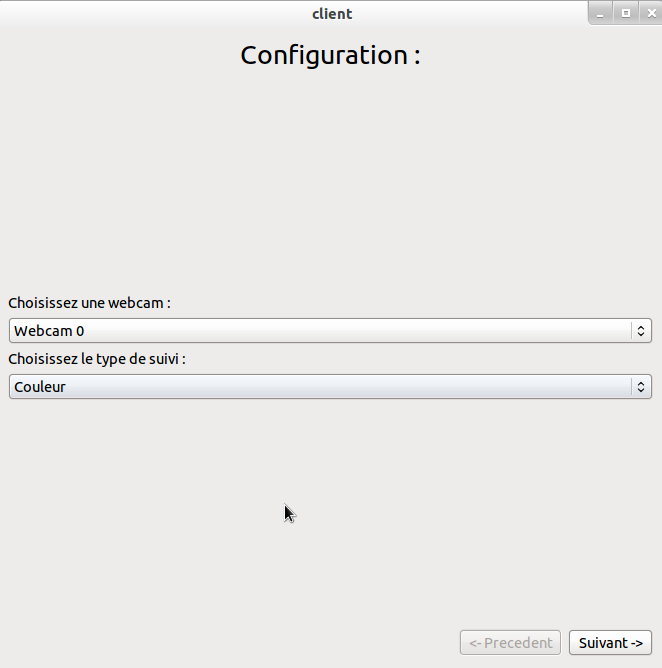
\includegraphics[scale=0.35]{../images/Capture6.png}\\
						\caption{Choix webcam/type track}
						\label{Choix webcam/type track}
				\end{figure}
				\paragraph{}
				La première liste déroulante permet le choix de la webcam à utiliser pour la capture, la seconde la sélection de la méthode de track parmi :
				\begin{itemize}
					\item Suivi par modèle
					\item Suivi par couleur, barycentre simple
					\item Suivi par couleur, composantes connexes
				\end{itemize}
				\paragraph{}
				Au niveau de la bibliothèque de suivi, ces listes servent à définir la sources des images servant au track, et à choisir le drapeau pour la fonction \textit{calibration}.
				\newpage
				\paragraph{}
				L'écran suivant permet quant à lui de sélectionner sur le retour image de la webcam l'objet à suivre, ou \textbf{curseur}.\\
				\begin{figure}[!h]
						\centering
						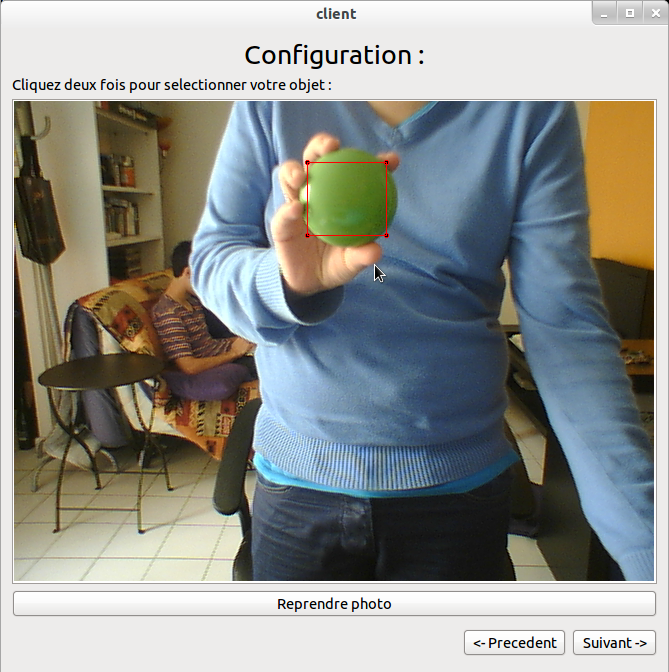
\includegraphics[scale=0.35]{../images/Capture1.png}\\
						\caption{Sélection du curseur}
						\label{Sélection du curseur}
				\end{figure}
				\paragraph{}
				Il suffit pour cela, par clics sur l'image, de créer une \textbf{boîte englobante}, ou hitbox, autour dudit curseur.
				Cet écran sert à récupérer les coordonnées de la hitbox nécessaire à l'\textbf{isolement} de l'objet pour le suivi par comparaison de modèle, ou à l'\textbf{extraction} de la couleur et de l'aire de l'objet pour les suivis par couleur.
				\newpage
				\paragraph{}
				Grâce à la précédente sélection, on affiche le \textbf{masque binaire} permettant de vérifier que l'objet a bien été reconnu. Les zones blanches sur l'image représentent les parties reconnues par l'application, le but étant alors d'avoir une zone blanche cohérente sur le curseur.
				\begin{figure}[!h]
						\centering
						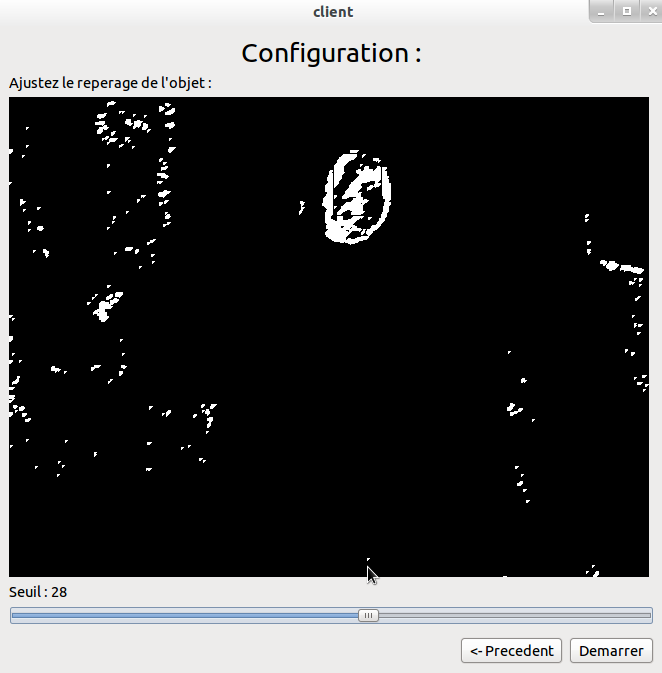
\includegraphics[scale=0.35]{../images/Capture2.png}\\
						\caption{Réglage du seuil}
						\label{Réglage du seuil}
				\end{figure}
				\paragraph{}
				La règlette permet d'affiner le masque binaire en augmentant ou diminuant le \textbf{seuil de tolérance} pour la reconnaissance de couleur.
				\paragraph{}
				Dans le cas du suivi par modèle, on affiche simplement le modèle qui sera utilisé pour le suivi.
				\begin{figure}[!h]
						\centering
						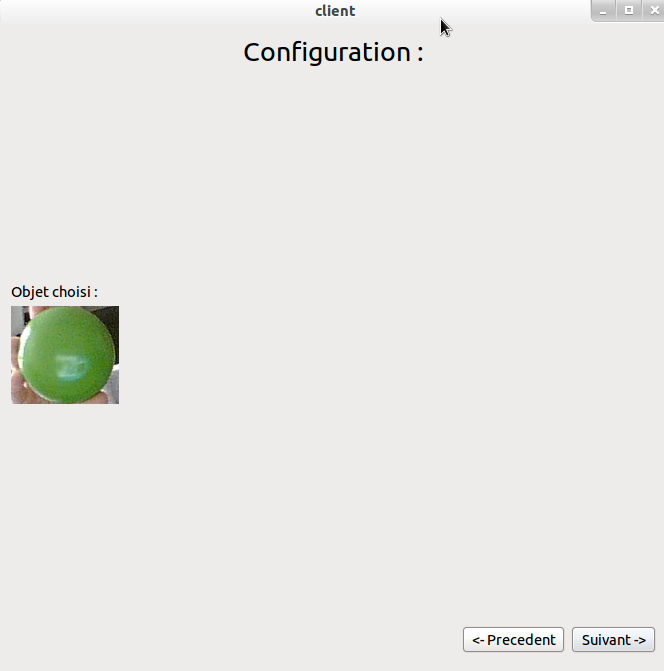
\includegraphics[scale=0.35]{../images/Capture7.png}\\
						\caption{Contrôle du modèle}
						\label{Contrôle du modèle}
				\end{figure}
				\newpage
				\paragraph{}
				Enfin, le dernier écran de l'étalonnage permet de décider si la session de dessin est à un seul utilisateur, en \textbf{local}, ou à plusieurs via le \textbf{mode réseau}.
				\begin{figure}[!h]
						\centering
						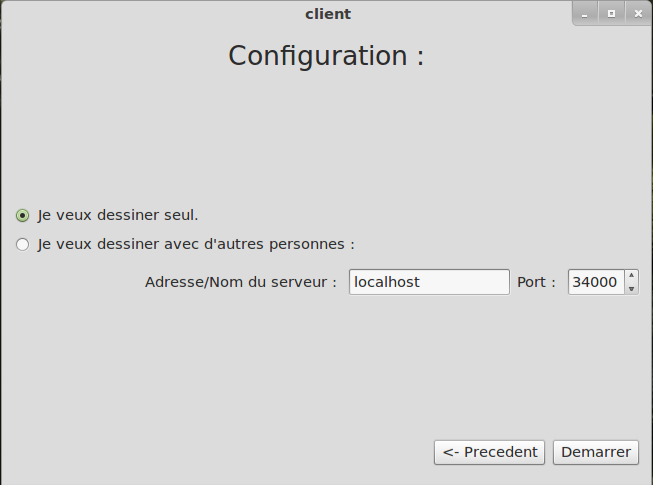
\includegraphics[scale=0.4]{../images/capture_choix.png}\\
						\caption{Sélecteur Local/Réseau}
						\label{Sélecteur Local/Réseau}
				\end{figure}
				\paragraph{}
				Si le dessin se fait en réseau, il faut renseigner l'adresse et le port du serveur hébergeant la session, c'est la seule différence par rapport au mode local du point de vue de l'interface.
				\newpage
			\subsection{Dessin}
			L'interface de dessin est conçue pour être très simple et intuitive : l'écran à gauche représente l'état courant du dessin (le tableau donc), et à droite l'utilisateur peut voir un aperçu du flux vidéo en temps réel. \\
			Le dessin est donc relativement facile et intuitif, on voit directement l'effet d'un mouvement de l'objet suivi. \\
			Le menu en haut permet quant à lui de sélectionner différentes actions à la souris, tandis qu'une interface gestuelle permet d'effectuer les actions liées au dessin sans utiliser la souris. \\
			L'interface gestuelle permet de choisir la gomme et les couleurs rouge, vert, bleu et noire. Elle permet également de diminuer ou de grossir la taille du pinceau, et enfin offre un aperçu de la couleur courante. \\
			Cette interface ne contient que des fonctionnalités très basiques pour des raisons exprimées précédemment. \\
				\begin{figure}[!h]
						\centering
						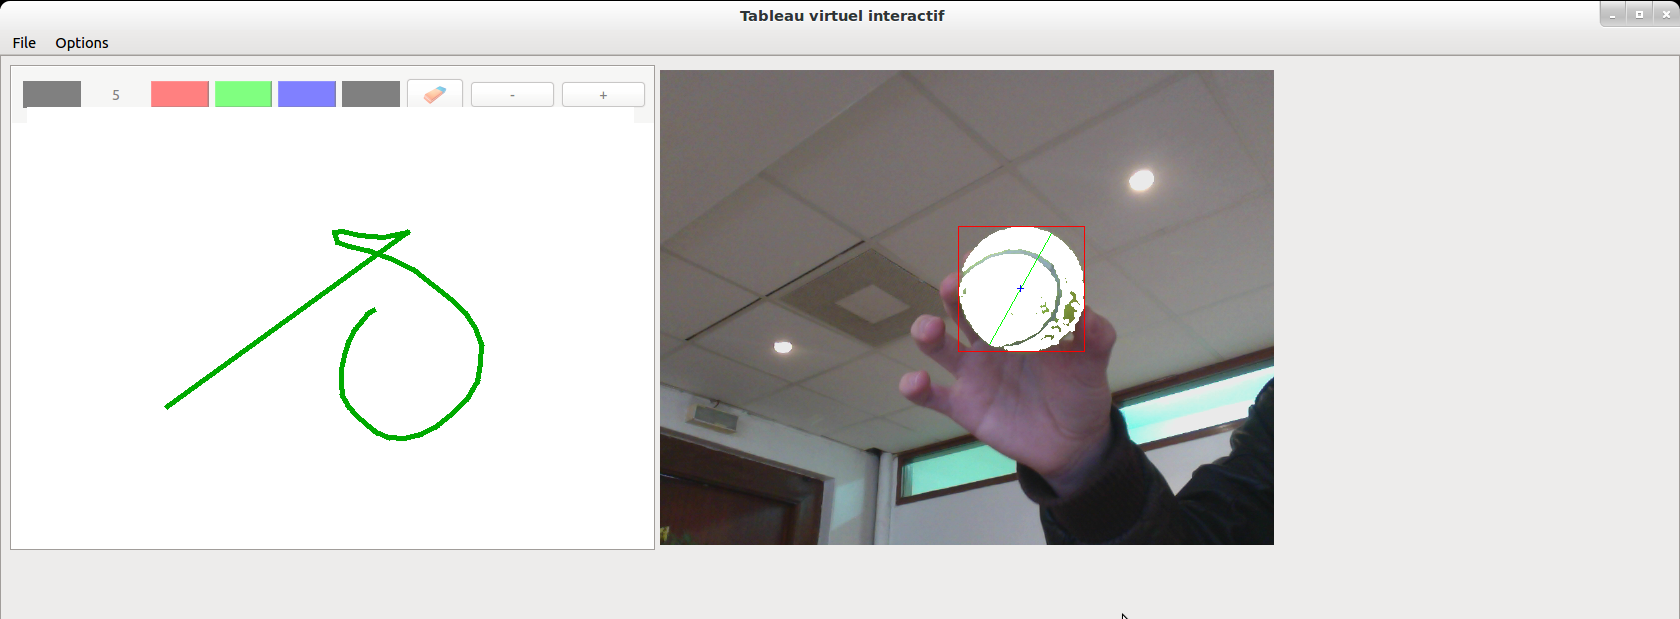
\includegraphics[scale=0.3]{capture.png}\\
						\caption{Interface de dessin}
						\label{Interface de dessin}
				\end{figure}
				\newpage
				Le sélecteur de couleur permet de choisir très précisément la couleur voulue. \\
				\begin{figure}[!h]
						\centering
						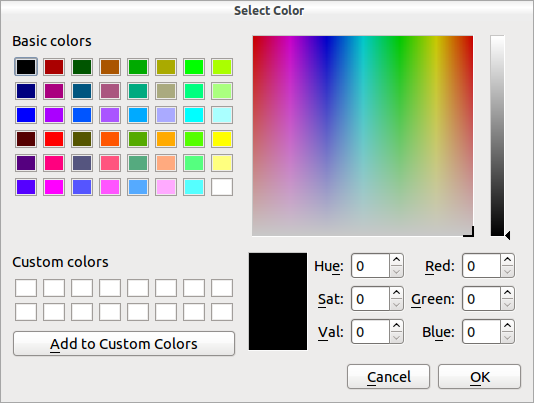
\includegraphics[scale=0.4]{../images/colorpicker.png}\\
						\caption{Selecteur de couleur}
						\label{Selecteur de couleur}
				\end{figure}
				
				Le menu offre des fonctionnalités sur le dessin comme le nettoyage total du tableau, le passage en plein écran ou encore l'accès au sélecteur de couleurs. \\
				\begin{figure}[!h]
						\centering
						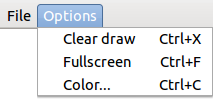
\includegraphics[scale=0.4]{../images/menu.png}\\
						\caption{Menu}
						\label{Menu}
				\end{figure}
				
				La fenêtre d'exportation permet de sauvegarder à l'endroit voulue l'image provenant du tableau, le format de base utilisé est le PNG, le chemin d'enregistrement du fichier est par défaut dans le répertoire home/ sous LINUX. \\
				\begin{figure}[!h]
						\centering
						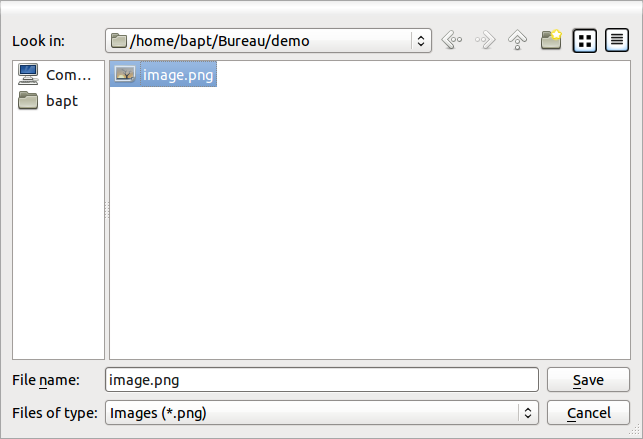
\includegraphics[scale=0.4]{../images/export.png}\\
						\caption{Export}
						\label{Export}
				\end{figure}
				\newpage
		\section{Serveur}
		Le serveur ne possède pas d'interface graphique, les résultats présentés seront donc essentiellement textuels. \\
		Son fonctionnement est simple, il se charge de stocker les clients, et de recevoir et traiter leurs ordres.\\
		En pratique cela est fait grâce à une classe \textbf{PackageManager} qui se charge de recevoir et découper les paquets des clients. Une fois le paquet découpé il est traité selon le schéma présenté plus haut. \\
		Le serveur a donc essentiellement un but de synchronisation : il reçoit les paquets, s'assure que chaque client possède bien le même dessin, et partage les points dessinés avec tous les clients (y compris les nouveaux arrivants qui récupèrent directement le tableau). \\
		\begin{figure}[!h]
			\centering
			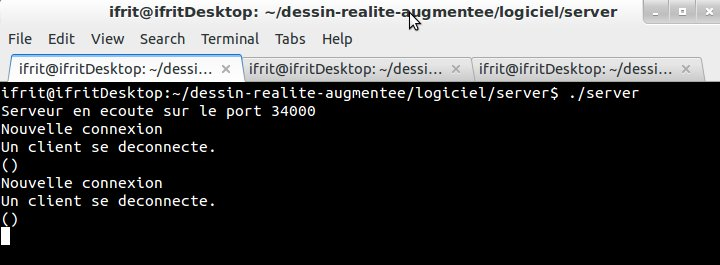
\includegraphics[scale=0.6]{../images/captureServer.jpg}\\
			\caption{Interface terminal du Serveur}
			\label{Interface terminal du Serveur}
		\end{figure}
		
		\newpage
		\section{Comparatif des méthodes de suivi}
		Cette partie va nous permettre de comparer les différentes méthodes de suivi implantées dans notre bibliothèque. Nous verrons en effet que celles-ci ne se valent pas toutes, et qu'il peut être préférable de choisir l'une ou l'autre en fonction du contexte.
				        \begin{figure}[h]
				\Large{
				\begin{center}
				\begin{tabular}{|l|c|c|c|}
				\hline
				\backslashbox{Caractéristique}{\quad Méthode}& Modèle  &Couleur : CC & Couleur : Simple  \\
				\hline
				Vitesse & -& + & ++ \\
				\hline
				Précision &++&++&+\\
				\hline
				Linéarité du suivi&-&+&+\\
				\hline
				Variété curseur &++&+&++\\
				\hline
				Souplesse, adaptation & - - & + &+\\
				\hline
				Sensibilité environnement &++&-&- -\\
				\hline
				Action &Non & Oui & Oui \\
				\hline
				\end{tabular}
				\end{center}
				\caption{Comparatif des différentes solutions de suivi}
				\label{tableau comparatif}}
				\end{figure}
				
			Les deux premières caractéristiques qu'il est intéressant de comparer sont la vitesse et la précision du suivi. En effet, ce vont être les deux spécificités que va rechercher l'utilisateur de la bibliothèque. Dans les trois méthodes présentées, on remarque une tendance assez intuitve, qui est qu'une méthode plus précise a tendance à être plus lente, de part des calculs plus complexes.
			\paragraph{}
			La linéarité du suivi indique la résistance d'une méthode aux pertes ponctuelles du curseur. C'est un peu le pendant de la précision d'une méthode : à vouloir être trop restrictif dans la détection du curseur, il y a le risque de ne pas le détecter même lorsqu'il est présent sur l'image.
			\paragraph{}
			La variété du curseur représente l'éventail des possibilités qu'a l'utilisateur quant au choix de l'objet qu'il souhaite suivre. Comme nous avons pu le signaler, le track par modèle permet le suivi de tout type d'objet quand les tracks par couleurs peuvent être limités dans l'utilisation d'objet fortement multicolores.
			\paragraph{}
			La souplesse permet d'évaluer la robustesse du suivi d'un objet si celui-ci est modifié durant le suivi. Cette modification, qui peut être due à un problème d'éclairage ou plus simplement à une rotation de l'objet par exemple, impacte fortement sur l'efficacité du suivi par modèle. On pourrait palier à ce problème en mettant en place un suivi avec apprentissage, qui pourrait prendre en compte les modifications progressives du curseur afin de perfectionner son efficacité.
			\paragraph{}
			La sensibilité à l'environnement est un point important à prendre en compte. En effet, lors de l'utilisation d'un suivi par couleur, il faut faire attention à ne pas suivre un objet dont la couleur serait identique au fond. De ce point de vue, le suivi par modèle impose une efficacité parfaite en étant capable de détecter un objet sur un fond d'une couleur presque similaire avec une forte précision.
			\paragraph{}
			La présence d'action indique si nous avons réussi à mettre en place une détection d'action, comme en utilisant la taille de l'objet dans les suivis par couleur.
		
		\newpage
		\section{Mise en production}
		La mise en production est quelque chose qui est souvent oublié par manque de temps, ou manque d'expériences, nous voulions dans le cadre du TER avoir un projet qui soit réellement abouti. \\
		
		\paragraph{Programmation et documentation\\} La première étape était de bien penser l'application, pour produire du code de qualité tout au long du projet, et ainsi d'avoir une bibliothèque réutilisable et un code compréhensible et extensible dans l'application. \\
		La bibliothèque est également entièrement documentée (cf annexe) à l'aide de docxygen, les fonctions sont donc compréhensibles et il est indiqué clairement les entrées et les sorties. \\
		
		\paragraph{Traduction \\} L'application est également traduite à l'aide d'un module dédié de Qt, selon la langue de la machine l'application est en français, ou en anglais pour toutes les autres langues. \\
		
		\paragraph{Packaging \\} Nous avons créé un .deb pour l'application, qui utilise le gestionnaire de paquets de Debian, les dépendances sont donc gérées et l'application est facilement installable sur les systèmes LINUX basés sur Debian. \\
		
	\chapter{Conclusion}
		\section{Difficultés rencontrées}
		Au cours de ce projet, nous avons rencontré des difficultés de plusieurs natures. Tout d'abord c'était un projet relativement long et compliqué par rapport à notre expérience, nous avons donc du nous préparer sur la gestion de ce projet. \\
		De plus une grande partie des difficultés réside dans des problèmes techniques (de conception, ou de programmation). \\
		
		\paragraph{Synchronisation \\}
		Pour effectuer ce travail, nous devions nous retrouver régulièrement pour être parfaitement au courant des évolutions du projet, pour se fixer de nouveaux objectifs, pour savoir où aller ou encore pour définir des buts concrets et atteignables. \\
		Nous avons aussi mis en place plusieurs outils techniques pour nous permettre de mettre en commun tout le code et les documents : nous avons utilisé un gestionnaire de version, ainsi que des outils d'éditions collaborative. \\
		Le fait d'avoir un groupe qui a déjà travaillé ensemble plusieurs fois sur des projets précédents nous a aussi aidé à etre rapidement efficace et à savoir quoi faire, c'est donc une difficulté que nous avons relativement bien surmontée. \\
		
		\paragraph{Technique \\}
		Nous avons également du nous former en parallèle au traitement de l'image par exemple. Nous avons trouvé plusieurs documents qui nous présentaient les grands principes avec différentes méthodes pour suivre des objets etc. Pour la partie bibliothèque il y avait beaucoup de formation, mais le TER coïncidait avec une UE traitement de l'image pour les IMAGINA, ce qui a aussi aidé. \\
		Une autre difficulté résidait dans la conception globale, pour avoir une architecture solide et avoir une application aboutie nous avons passé du temps à penser le projet pour pouvoir avancer vite par la suite. \\ C'est une partie où nous nous en sommes plûtot bien sortis, malgré le module réseau qui souffre encore de lenteurs et qui devrait donc être optimisé. \\
		
		Pour des problèmes plus concrets, nous avons également eu des difficultés liées à la gestion de la mémoire : la librairie OpenCV fournit des fonctions à allocations implicites, avec une gestion de la mémoire très particulière et une documentation assez légère. Nous nous sommes donc heurtés dans plusieurs phases du projet à repenser localement l'architecture pour éviter d'avoir trop de création d'objet et d'image qui n'étaient pas libérées. \\
		\newpage

		\section{Perspectives}
		Les perspectives peuvent se découper en deux parties qui seraient l'amélioration de l'existant et des fonctionnalités que nous n'avons pas pu faire, ou même auxquelles nous n'avions pas pensé avant un stade avancé du projet. \\
		
		\paragraph{Optimisations \\}
		Pour la partie bibliothèque il faudrait implémenter la détection d'action lors d'un suivi par forme. \\
		De manière générale il faudrait aussi réduire encore la dépendance vis à vis de l'environnement. \\
		Côté application le principal problème réside dans les lenteurs du mode réseau, une solution serait peut être d'échanger moins de points, ou encore de faire des systèmes de mémoires tampons pour avoir un nombre d'envois plus réduit. \\
		
		Pour le projet global, les performances sont assez bonnes, mais nous pourrions aussi essayer de les améliorer encore pour plus de rapidité. \\ 
		
		\paragraph{Nouvelles fonctionnalités \\}
		Une fonctionnalité intéressante serait de suivre plusieurs objets en même temps, pour dessiner avec plusieurs curseurs et également d'avoir d'autres actions détectées. Lors de la soutenance un membre du jury parlait d'un système permettant de zoomer avec deux curseurs, à la manière du zoom sur les téléphones et tablettes avec deux doigts. \\
Ces deux fonctionnalités sont intéressantes et pourraient être ajoutées sans changements de la bibliothèque. \\	
		
		\section{Conclusion}
		Ce TER a donc permis de faire un travail de recherche et d'analyse qui a abouti à un résultat concret pour un projet qui a encore des perspectives d'évolutions.
		Cela a donc été une expérience très enrichissante qui nous a permis de mener un projet de A à Z. Ceci a inclus sa proposition, la rédaction du cahier des charges, l'analyse et le développement sans oublier la mise en production. \\
		Tout ceci était relativement nouveau pour nous tous, ce projet est donc une réussite avec de nombreux objectifs initiaux qui ont été atteints. Nous avons également réussi à gérer notre groupe de projet de manière à répartir correctement le travail en fonctionnant en deux sous-équipes. \\ 
	
	\chapter{Références}
	
	\paragraph{Documents de recherches :}
	ces divers documents nous ont servi dans la partie d'analyse et de réflexion du projet ce qui a permis de savoir où aller, et donc de développer plus efficacement dans un second temps. \\
	Ces documents ont surtout permis de comprendre le domaine du traitement de l'image avec ce que cela implique, ainsi que des applications possibles. Plus généralement ils nous permettaient de découvrir le monde de la recherche en lisant des articles spécifiques et/ou des thèses. \\
		\begin{itemize}
			\item \it{Real-time viewpoint-invariant hand localization with cluttered backgrounds} \\
			Enver Sangineto, Marco Cupelli.
			\begin{verbatim}
			http://www.sciencedirect.com/science/article/pii/S026288561100120X
			\end{verbatim}
			\item \it{Vision par ordinateur pour l’interaction homme-machine fortement couplée}\\
			Thèse de françois Bérard sur un sujet proche avec beaucoup d'informations
			\begin{verbatim}
			http://hal.inria.fr/docs/00/04/61/56/PDF/tel-00004804.pdf
			\end{verbatim}
			\item \it{Defining Search Areas to Localize Limbs in Body Motion Analysis} \\
			Thomas Foures, Philippe Joly.
			\item \it{Indexation de la vidéo par le costume.}\\ 
			Thèse de doctorat, Université Paul Sabatier Toulouse, Gaël Jaffré.
			\begin{verbatim}
			http://www.irit.fr/recherches/SAMOVA/pageautomatic-character-labelling-in-videos.html
			\end{verbatim}
		\end{itemize}
			
		\paragraph{Documents de programmation :}
		ces documents ont servis de référence pour développer avec OpenCV, ainsi que d'apprendre des concepts non spécifiques à une librairie dans le domaine du traitement de l'image. \\
			\begin{itemize}
			\item \it{Vision par ordinateur : Outils fondamentaux} \\
			Radu HORAUD (CNRS) et Olivier MONGA (INRIA)
			\begin{verbatim}
			http://hal.archives-ouvertes.fr/docs/00/59/00/49/PDF/VO-HoraudMonga.pdf
			\end{verbatim}
			\item Learning Open CV \\
			 Gary Bradski et Adrian Kaehler
			\item Open Cv 2 Computer Vision Application Programming Cookbook\\
			Robert Laganière
			\end{itemize}
	
	\part{Annexes}
	\appendix
		\chapter{Documentation de la bibliothèque}
		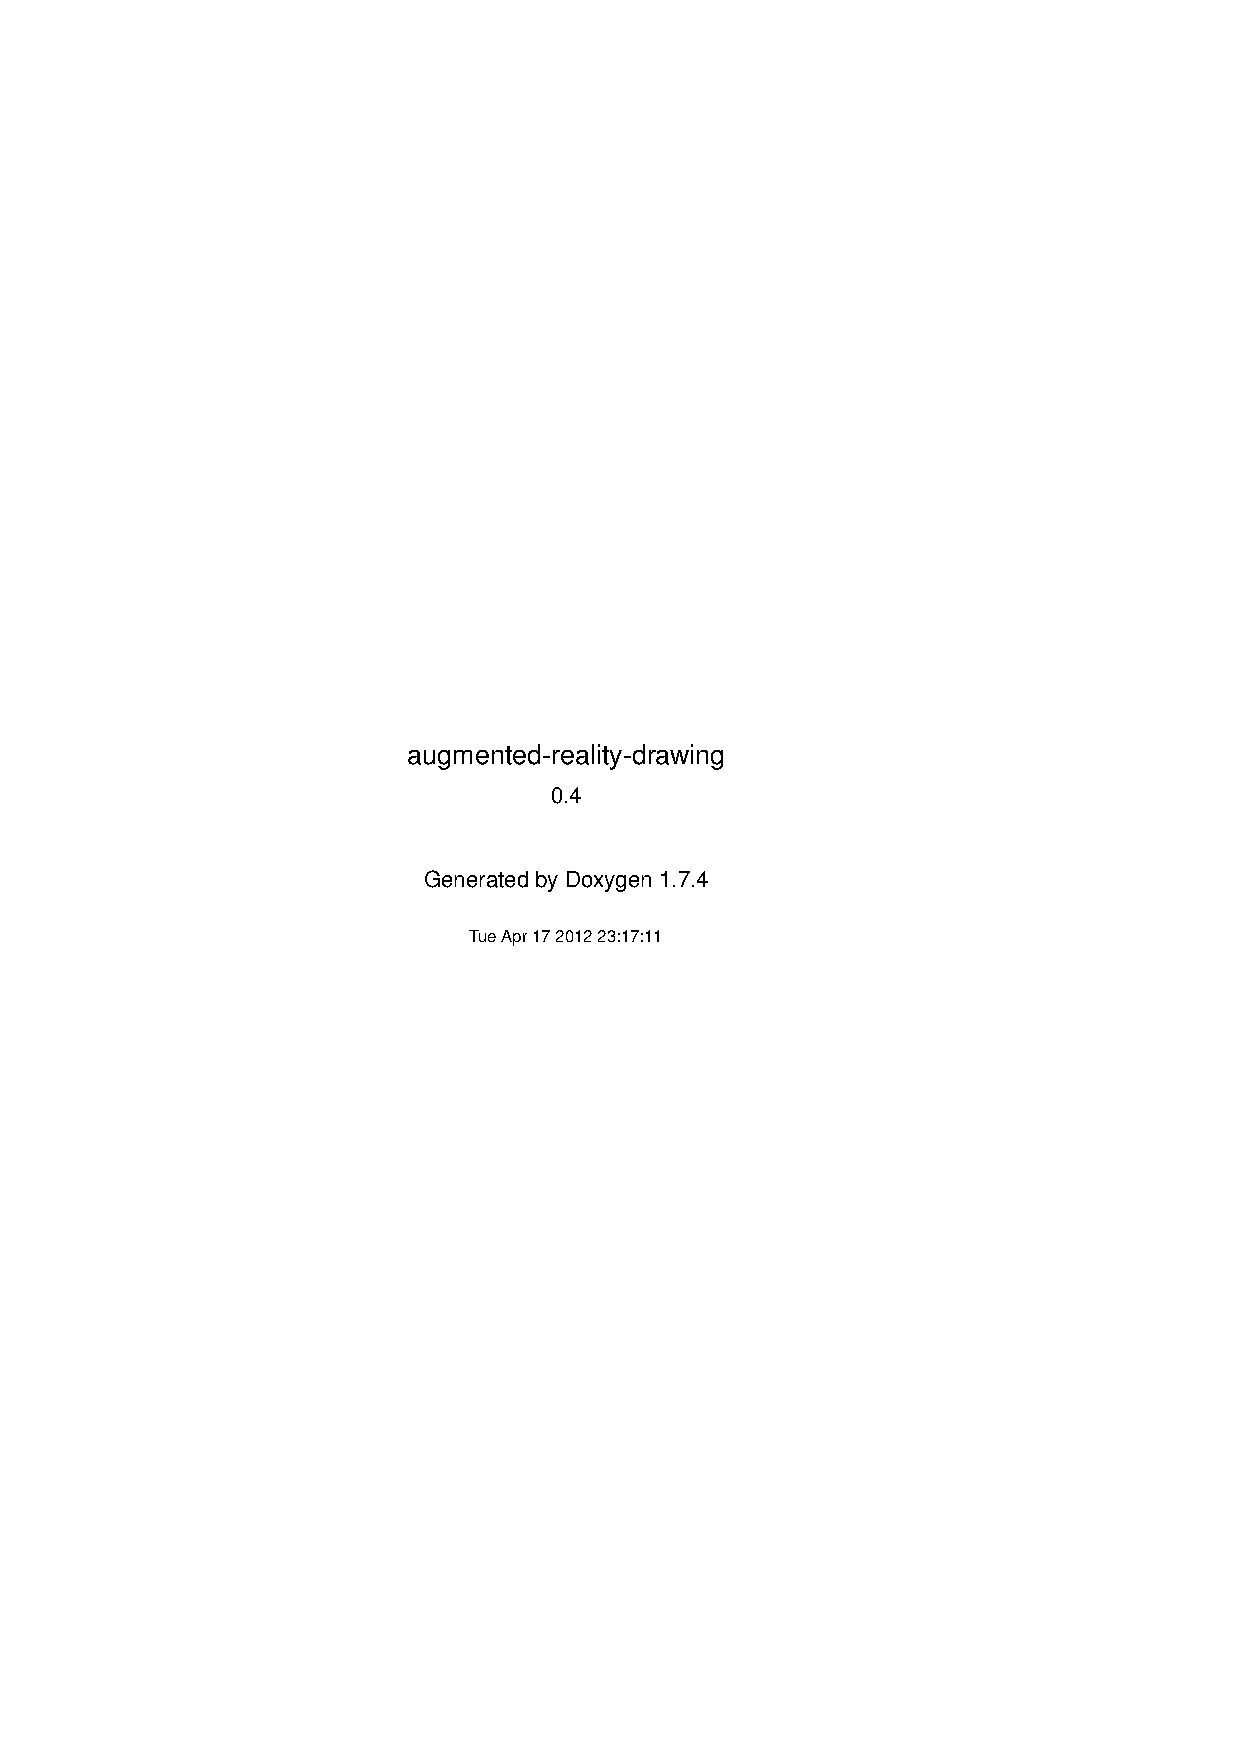
\includepdf[pages = {1-15}]{../code-doc/refman.pdf}
\end{document}
